\documentclass[aspectratio=169,11pt]{beamer}

\newcommand{\currentpart}{1}
% ============================================================================
% Quantitative Research -- shared preamble for all five slide decks
%
% Every deck starts with
%     \documentclass[aspectratio=169,11pt]{beamer}
%     % ============================================================================
% Quantitative Research -- shared preamble for all five slide decks
%
% Every deck starts with
%     \documentclass[aspectratio=169,11pt]{beamer}
%     % ============================================================================
% Quantitative Research -- shared preamble for all five slide decks
%
% Every deck starts with
%     \documentclass[aspectratio=169,11pt]{beamer}
%     \input{../common/preamble.tex}
%     \newcommand{\currentpart}{<k>}
% so that layout, colours, boxes and code listings are identical everywhere.
% ============================================================================

% ======================== Packages ========================
\usepackage[utf8]{inputenc}
\usepackage[T1]{fontenc}
\usepackage[english]{babel}
\usepackage{graphicx}
\usepackage{booktabs}
\usepackage{amsmath,amssymb,amsfonts}
\usepackage{mathtools}
\usepackage{xcolor}
\usepackage{colortbl}
\usepackage{array}
\usepackage{multicol}
\usepackage{verbatim}          % provides the comment environment
\usepackage{tikz}
\usepackage{pgfplots}
\pgfplotsset{compat=1.18}
\usetikzlibrary{arrows.meta,positioning,fit,backgrounds,shapes.geometric,calc,decorations.pathreplacing}
\usepackage{listings}
\usepackage{hyperref}
\usepackage{pgfpages}          % notes on a second screen (only if enabled)

% ======================== Speaker notes (talk-tracks) ========================
% The decks compile WITHOUT notes by default. To get a version with the
% talk-tracks, uncomment exactly ONE of the lines below and recompile:
% \setbeameroption{show notes}                          % notes as separate pages
% \setbeameroption{show notes on second screen=right}   % slides left, notes right

% ======================== Math fonts ========================
% Beamer typesets text in sans serif; make \mathrm and \mathbf match it
% (otherwise SE, TP, RSS print in serif and \mathbf falls back to non-bold).
\renewcommand{\bfdefault}{bx}   % CM sans has bold extended (bx) only
\DeclareMathAlphabet{\mathrm}{T1}{cmss}{m}{n}
\DeclareMathAlphabet{\mathbf}{T1}{cmss}{bx}{n}
\SetMathAlphabet{\mathrm}{bold}{T1}{cmss}{bx}{n}
\SetMathAlphabet{\mathbf}{bold}{T1}{cmss}{bx}{n}
\SetSymbolFont{operators}{bold}{OT1}{cmss}{bx}{n}
% Beamer re-declares \mathrm at \begin{document}; re-apply the sans-serif version
\AtBeginDocument{\SetMathAlphabet{\mathrm}{normal}{T1}{cmss}{m}{n}%
                 \SetMathAlphabet{\mathrm}{bold}{T1}{cmss}{bx}{n}}

% ======================== Colour palette (matched to plots / Madrid) ========
\definecolor{hsbiblau}{HTML}{3333B2}
\definecolor{hsbiblaudunkel}{HTML}{1C1C6E}
\definecolor{hsbiorange}{HTML}{E69F00}
\definecolor{hsbigrau}{HTML}{9A9A9A}
\definecolor{hsbirot}{HTML}{C0392B}
\definecolor{hsbigruen}{HTML}{2E8B57}
\definecolor{hsbiviolett}{HTML}{8C3CA0}   % 4th comparison colour (e.g. candidate lines)

% ======================== Theme ========================
\usetheme{Madrid}
\usecolortheme{default}
\setbeamertemplate{navigation symbols}{}
\setbeamertemplate{blocks}[rounded][shadow=false]
\setbeamerfont{section in head/foot}{size=\tiny}

% Horizontal section navigation bar in the headline
\setbeamertemplate{headline}{%
  \leavevmode%
  \hbox{%
    \begin{beamercolorbox}[wd=\paperwidth,ht=2.5ex,dp=1.125ex]{section in head/foot}%
      \scriptsize\insertsectionnavigationhorizontal{\paperwidth}{}{\hskip0pt plus1filll}%
    \end{beamercolorbox}%
  }%
}

% Footline: lecture part, current section (if any) and slide number
\newcommand{\footsection}{%
  \setbox0=\hbox{\insertsection}%
  \ifdim\wd0>0pt\ \textbar\ \insertsection\fi}
\setbeamertemplate{footline}{%
  \leavevmode%
  \hbox{%
  \begin{beamercolorbox}[wd=\paperwidth,ht=2.5ex,dp=1.125ex]{author in head/foot}%
    \hspace*{2em}Part~\currentpart\footsection\hfill\insertframenumber{}/\inserttotalframenumber\hspace*{2em}%
  \end{beamercolorbox}%
  }%
}

% Automatic section overview slide. Decks with many sections define
%   \newcommand{\overviewleft}{1-4}\newcommand{\overviewright}{5-8}
% before \begin{document} to get a two-column overview.
\newcommand{\overviewtoc}[1]{%
  \tableofcontents[currentsection,sectionstyle=show/shaded,
                   subsectionstyle=show/show/hide,sections={#1}]}
\newcommand{\sectionoverview}{%
  \ifdefined\overviewleft
    \begin{columns}[T]
      \column{0.49\textwidth}\overviewtoc{\overviewleft}
      \column{0.49\textwidth}\overviewtoc{\overviewright}
    \end{columns}%
  \else
    \tableofcontents[currentsection,sectionstyle=show/shaded,
                     subsectionstyle=show/show/hide]%
  \fi}
\AtBeginSection[]{%
  \begin{frame}{Overview}
    \scriptsize
    \sectionoverview
  \end{frame}%
}

% ======================== Python listing style ========================
\lstdefinestyle{Pystyle}{
  language=Python,
  basicstyle=\ttfamily\footnotesize,
  keywordstyle=\color{hsbiblau},
  commentstyle=\color{hsbigrau}\itshape,
  stringstyle=\color{teal},
  showstringspaces=false,
  literate={~}{{$\sim$}}1
           {–}{{--}}1 {—}{{---}}1 {ä}{{\"a}}1 {ö}{{\"o}}1 {ü}{{\"u}}1
           {Ä}{{\"A}}1 {Ö}{{\"O}}1 {Ü}{{\"U}}1 {ß}{{\ss}}1 {é}{{\'e}}1,
  upquote=true,
  columns=fixed, basewidth=0.5em
}
% Plain style for printed Python output (fixed columns keep tables aligned)
\lstdefinestyle{Pyout}{
  language={},
  basicstyle=\ttfamily\scriptsize,
  keywordstyle={}, commentstyle={}, stringstyle={},
  columns=fixed, keepspaces=true, basewidth=0.52em,
  showstringspaces=false,
  upquote=true,
  literate={~}{{$\sim$}}1 {–}{{--}}1 {—}{{---}}1 {‘}{{`}}1 {’}{{'}}1,
}
\lstset{style=Pystyle}

% ======================== Custom commands / styles ========================
\newcommand{\kernaussage}[1]{\begin{alertblock}{Key takeaway}#1\end{alertblock}}
\newcommand{\inworten}[1]{{\small\textbf{\textcolor{hsbiblaudunkel}{In words:}}~#1}}
\newcommand{\guidingquestion}[1]{\begin{exampleblock}{Guiding question}#1\end{exampleblock}}
\newcommand{\appendixnote}[1]{\par\vfill\vspace{-1.6ex}\hfill{\scriptsize\itshape\textcolor{hsbiblau}{$\rightarrow$ Appendix: #1}}\par\vspace{-1ex}}
\newcommand{\sourcenote}[1]{\vfill\hfill{\tiny\itshape\color{gray}Source: #1}\par}

% Companion notebooks (Jupyter / Google Colab). Every deck defines
%     \newcommand{\notebookpath}{Part_k_<Topic>/Part_k_<Topic>.ipynb}
% \trynotebook{<notebook section>} prints a small clickable pointer at the
% bottom right of a frame that opens the deck's notebook in Google Colab
% (the same notebook lies next to the .tex file for local Jupyter use).
\newcommand{\colaburl}{https://colab.research.google.com/github/ChrisW09/Quantitative-Research-Methods/blob/main/}
\newcommand{\trynotebook}[1]{\par\vfill\vspace{-1.6ex}\hfill{\scriptsize\href{\colaburl\notebookpath}{\textcolor{hsbiorange!85!black}{$\blacktriangleright$\ \textbf{Try it yourself:} notebook, #1 \ -- open in Colab}}}\par\vspace{-1ex}}

% Reusable TikZ styles for concept diagrams
\tikzset{
  flowbox/.style={rounded corners, draw=hsbiblaudunkel, very thick,
                  fill=hsbiblau!10, align=center, inner sep=5pt, minimum height=8mm},
  flowboxo/.style={rounded corners, draw=hsbiorange!85!black, very thick,
                   fill=hsbiorange!18, align=center, inner sep=5pt, minimum height=8mm},
  flowboxg/.style={rounded corners, draw=hsbigrau!90!black, very thick,
                   fill=hsbigrau!15, align=center, inner sep=5pt, minimum height=8mm},
  flowarr/.style={-{Latex[length=2.6mm,width=2mm]}, line width=1pt, draw=hsbiblaudunkel},
}

% ======================== Course overview (same slide in every deck) ========
% \courseoverview highlights the part given by \currentpart.
\newcommand{\cpart}[2]{%
  \ifnum\currentpart=#1\relax
    \textcolor{hsbiblau}{\textbf{#2}}%
  \else
    #2%
  \fi}
\newcommand{\courseoverview}{%
\begin{frame}{The lecture at a glance}
  \begin{center}
    \small\renewcommand{\arraystretch}{1.15}
    \begin{tabular}{@{}l l >{\raggedright\arraybackslash}p{9.2cm}@{}}
      \toprule
      & \textbf{Part} & \textbf{Content} \\
      \midrule
      \ifnum\currentpart=1 $\blacktriangleright$\fi & \cpart{1}{1 -- Descriptive Statistics}
        & \cpart{1}{Basic concepts, levels of measurement, frequencies, measures of central tendency and dispersion} \\
      \ifnum\currentpart=2 $\blacktriangleright$\fi & \cpart{2}{2 -- Graphical Representations}
        & \cpart{2}{Empirical CDF, histogram, boxplot} \\
      \ifnum\currentpart=3 $\blacktriangleright$\fi & \cpart{3}{3 -- Statistical Inference}
        & \cpart{3}{Normal distribution and CLT, confidence intervals, sample size, hypothesis tests, $p$-values, one-sided tests, types of error} \\
      \ifnum\currentpart=4 $\blacktriangleright$\fi & \cpart{4}{4 -- Regression}
        & \cpart{4}{Correlation, least squares, goodness of fit, inference for regression, multiple regression (appendix: residual analysis)} \\
      \ifnum\currentpart=5 $\blacktriangleright$\fi & \cpart{5}{5 -- Classification}
        & \cpart{5}{Conditional probability, logistic regression, classification rules, confusion matrix, base rates, ROC/AUC, Bayes classifiers} \\
      \bottomrule
    \end{tabular}
  \end{center}
  \begin{center}
    \footnotesize All analyses are carried out in \textbf{Python} (NumPy,
    pandas, SciPy, statsmodels, matplotlib); every deck comes with a Python
    script that reproduces its numbers and a Jupyter notebook with all
    examples and exercises -- also in Google Colab.
  \end{center}
\end{frame}}

% ======================== Title information (shared) ========================
\title{Quantitative Research}
\author{Prof.\ Dr.\ Christoph Weisser}
\institute{}
\date{}   % must stay explicitly empty -- otherwise Beamer prints today's date

\graphicspath{{images/}}

%     \newcommand{\currentpart}{<k>}
% so that layout, colours, boxes and code listings are identical everywhere.
% ============================================================================

% ======================== Packages ========================
\usepackage[utf8]{inputenc}
\usepackage[T1]{fontenc}
\usepackage[english]{babel}
\usepackage{graphicx}
\usepackage{booktabs}
\usepackage{amsmath,amssymb,amsfonts}
\usepackage{mathtools}
\usepackage{xcolor}
\usepackage{colortbl}
\usepackage{array}
\usepackage{multicol}
\usepackage{verbatim}          % provides the comment environment
\usepackage{tikz}
\usepackage{pgfplots}
\pgfplotsset{compat=1.18}
\usetikzlibrary{arrows.meta,positioning,fit,backgrounds,shapes.geometric,calc,decorations.pathreplacing}
\usepackage{listings}
\usepackage{hyperref}
\usepackage{pgfpages}          % notes on a second screen (only if enabled)

% ======================== Speaker notes (talk-tracks) ========================
% The decks compile WITHOUT notes by default. To get a version with the
% talk-tracks, uncomment exactly ONE of the lines below and recompile:
% \setbeameroption{show notes}                          % notes as separate pages
% \setbeameroption{show notes on second screen=right}   % slides left, notes right

% ======================== Math fonts ========================
% Beamer typesets text in sans serif; make \mathrm and \mathbf match it
% (otherwise SE, TP, RSS print in serif and \mathbf falls back to non-bold).
\renewcommand{\bfdefault}{bx}   % CM sans has bold extended (bx) only
\DeclareMathAlphabet{\mathrm}{T1}{cmss}{m}{n}
\DeclareMathAlphabet{\mathbf}{T1}{cmss}{bx}{n}
\SetMathAlphabet{\mathrm}{bold}{T1}{cmss}{bx}{n}
\SetMathAlphabet{\mathbf}{bold}{T1}{cmss}{bx}{n}
\SetSymbolFont{operators}{bold}{OT1}{cmss}{bx}{n}
% Beamer re-declares \mathrm at \begin{document}; re-apply the sans-serif version
\AtBeginDocument{\SetMathAlphabet{\mathrm}{normal}{T1}{cmss}{m}{n}%
                 \SetMathAlphabet{\mathrm}{bold}{T1}{cmss}{bx}{n}}

% ======================== Colour palette (matched to plots / Madrid) ========
\definecolor{hsbiblau}{HTML}{3333B2}
\definecolor{hsbiblaudunkel}{HTML}{1C1C6E}
\definecolor{hsbiorange}{HTML}{E69F00}
\definecolor{hsbigrau}{HTML}{9A9A9A}
\definecolor{hsbirot}{HTML}{C0392B}
\definecolor{hsbigruen}{HTML}{2E8B57}
\definecolor{hsbiviolett}{HTML}{8C3CA0}   % 4th comparison colour (e.g. candidate lines)

% ======================== Theme ========================
\usetheme{Madrid}
\usecolortheme{default}
\setbeamertemplate{navigation symbols}{}
\setbeamertemplate{blocks}[rounded][shadow=false]
\setbeamerfont{section in head/foot}{size=\tiny}

% Horizontal section navigation bar in the headline
\setbeamertemplate{headline}{%
  \leavevmode%
  \hbox{%
    \begin{beamercolorbox}[wd=\paperwidth,ht=2.5ex,dp=1.125ex]{section in head/foot}%
      \scriptsize\insertsectionnavigationhorizontal{\paperwidth}{}{\hskip0pt plus1filll}%
    \end{beamercolorbox}%
  }%
}

% Footline: lecture part, current section (if any) and slide number
\newcommand{\footsection}{%
  \setbox0=\hbox{\insertsection}%
  \ifdim\wd0>0pt\ \textbar\ \insertsection\fi}
\setbeamertemplate{footline}{%
  \leavevmode%
  \hbox{%
  \begin{beamercolorbox}[wd=\paperwidth,ht=2.5ex,dp=1.125ex]{author in head/foot}%
    \hspace*{2em}Part~\currentpart\footsection\hfill\insertframenumber{}/\inserttotalframenumber\hspace*{2em}%
  \end{beamercolorbox}%
  }%
}

% Automatic section overview slide. Decks with many sections define
%   \newcommand{\overviewleft}{1-4}\newcommand{\overviewright}{5-8}
% before \begin{document} to get a two-column overview.
\newcommand{\overviewtoc}[1]{%
  \tableofcontents[currentsection,sectionstyle=show/shaded,
                   subsectionstyle=show/show/hide,sections={#1}]}
\newcommand{\sectionoverview}{%
  \ifdefined\overviewleft
    \begin{columns}[T]
      \column{0.49\textwidth}\overviewtoc{\overviewleft}
      \column{0.49\textwidth}\overviewtoc{\overviewright}
    \end{columns}%
  \else
    \tableofcontents[currentsection,sectionstyle=show/shaded,
                     subsectionstyle=show/show/hide]%
  \fi}
\AtBeginSection[]{%
  \begin{frame}{Overview}
    \scriptsize
    \sectionoverview
  \end{frame}%
}

% ======================== Python listing style ========================
\lstdefinestyle{Pystyle}{
  language=Python,
  basicstyle=\ttfamily\footnotesize,
  keywordstyle=\color{hsbiblau},
  commentstyle=\color{hsbigrau}\itshape,
  stringstyle=\color{teal},
  showstringspaces=false,
  literate={~}{{$\sim$}}1
           {–}{{--}}1 {—}{{---}}1 {ä}{{\"a}}1 {ö}{{\"o}}1 {ü}{{\"u}}1
           {Ä}{{\"A}}1 {Ö}{{\"O}}1 {Ü}{{\"U}}1 {ß}{{\ss}}1 {é}{{\'e}}1,
  upquote=true,
  columns=fixed, basewidth=0.5em
}
% Plain style for printed Python output (fixed columns keep tables aligned)
\lstdefinestyle{Pyout}{
  language={},
  basicstyle=\ttfamily\scriptsize,
  keywordstyle={}, commentstyle={}, stringstyle={},
  columns=fixed, keepspaces=true, basewidth=0.52em,
  showstringspaces=false,
  upquote=true,
  literate={~}{{$\sim$}}1 {–}{{--}}1 {—}{{---}}1 {‘}{{`}}1 {’}{{'}}1,
}
\lstset{style=Pystyle}

% ======================== Custom commands / styles ========================
\newcommand{\kernaussage}[1]{\begin{alertblock}{Key takeaway}#1\end{alertblock}}
\newcommand{\inworten}[1]{{\small\textbf{\textcolor{hsbiblaudunkel}{In words:}}~#1}}
\newcommand{\guidingquestion}[1]{\begin{exampleblock}{Guiding question}#1\end{exampleblock}}
\newcommand{\appendixnote}[1]{\par\vfill\vspace{-1.6ex}\hfill{\scriptsize\itshape\textcolor{hsbiblau}{$\rightarrow$ Appendix: #1}}\par\vspace{-1ex}}
\newcommand{\sourcenote}[1]{\vfill\hfill{\tiny\itshape\color{gray}Source: #1}\par}

% Companion notebooks (Jupyter / Google Colab). Every deck defines
%     \newcommand{\notebookpath}{Part_k_<Topic>/Part_k_<Topic>.ipynb}
% \trynotebook{<notebook section>} prints a small clickable pointer at the
% bottom right of a frame that opens the deck's notebook in Google Colab
% (the same notebook lies next to the .tex file for local Jupyter use).
\newcommand{\colaburl}{https://colab.research.google.com/github/ChrisW09/Quantitative-Research-Methods/blob/main/}
\newcommand{\trynotebook}[1]{\par\vfill\vspace{-1.6ex}\hfill{\scriptsize\href{\colaburl\notebookpath}{\textcolor{hsbiorange!85!black}{$\blacktriangleright$\ \textbf{Try it yourself:} notebook, #1 \ -- open in Colab}}}\par\vspace{-1ex}}

% Reusable TikZ styles for concept diagrams
\tikzset{
  flowbox/.style={rounded corners, draw=hsbiblaudunkel, very thick,
                  fill=hsbiblau!10, align=center, inner sep=5pt, minimum height=8mm},
  flowboxo/.style={rounded corners, draw=hsbiorange!85!black, very thick,
                   fill=hsbiorange!18, align=center, inner sep=5pt, minimum height=8mm},
  flowboxg/.style={rounded corners, draw=hsbigrau!90!black, very thick,
                   fill=hsbigrau!15, align=center, inner sep=5pt, minimum height=8mm},
  flowarr/.style={-{Latex[length=2.6mm,width=2mm]}, line width=1pt, draw=hsbiblaudunkel},
}

% ======================== Course overview (same slide in every deck) ========
% \courseoverview highlights the part given by \currentpart.
\newcommand{\cpart}[2]{%
  \ifnum\currentpart=#1\relax
    \textcolor{hsbiblau}{\textbf{#2}}%
  \else
    #2%
  \fi}
\newcommand{\courseoverview}{%
\begin{frame}{The lecture at a glance}
  \begin{center}
    \small\renewcommand{\arraystretch}{1.15}
    \begin{tabular}{@{}l l >{\raggedright\arraybackslash}p{9.2cm}@{}}
      \toprule
      & \textbf{Part} & \textbf{Content} \\
      \midrule
      \ifnum\currentpart=1 $\blacktriangleright$\fi & \cpart{1}{1 -- Descriptive Statistics}
        & \cpart{1}{Basic concepts, levels of measurement, frequencies, measures of central tendency and dispersion} \\
      \ifnum\currentpart=2 $\blacktriangleright$\fi & \cpart{2}{2 -- Graphical Representations}
        & \cpart{2}{Empirical CDF, histogram, boxplot} \\
      \ifnum\currentpart=3 $\blacktriangleright$\fi & \cpart{3}{3 -- Statistical Inference}
        & \cpart{3}{Normal distribution and CLT, confidence intervals, sample size, hypothesis tests, $p$-values, one-sided tests, types of error} \\
      \ifnum\currentpart=4 $\blacktriangleright$\fi & \cpart{4}{4 -- Regression}
        & \cpart{4}{Correlation, least squares, goodness of fit, inference for regression, multiple regression (appendix: residual analysis)} \\
      \ifnum\currentpart=5 $\blacktriangleright$\fi & \cpart{5}{5 -- Classification}
        & \cpart{5}{Conditional probability, logistic regression, classification rules, confusion matrix, base rates, ROC/AUC, Bayes classifiers} \\
      \bottomrule
    \end{tabular}
  \end{center}
  \begin{center}
    \footnotesize All analyses are carried out in \textbf{Python} (NumPy,
    pandas, SciPy, statsmodels, matplotlib); every deck comes with a Python
    script that reproduces its numbers and a Jupyter notebook with all
    examples and exercises -- also in Google Colab.
  \end{center}
\end{frame}}

% ======================== Title information (shared) ========================
\title{Quantitative Research}
\author{Prof.\ Dr.\ Christoph Weisser}
\institute{}
\date{}   % must stay explicitly empty -- otherwise Beamer prints today's date

\graphicspath{{images/}}

%     \newcommand{\currentpart}{<k>}
% so that layout, colours, boxes and code listings are identical everywhere.
% ============================================================================

% ======================== Packages ========================
\usepackage[utf8]{inputenc}
\usepackage[T1]{fontenc}
\usepackage[english]{babel}
\usepackage{graphicx}
\usepackage{booktabs}
\usepackage{amsmath,amssymb,amsfonts}
\usepackage{mathtools}
\usepackage{xcolor}
\usepackage{colortbl}
\usepackage{array}
\usepackage{multicol}
\usepackage{verbatim}          % provides the comment environment
\usepackage{tikz}
\usepackage{pgfplots}
\pgfplotsset{compat=1.18}
\usetikzlibrary{arrows.meta,positioning,fit,backgrounds,shapes.geometric,calc,decorations.pathreplacing}
\usepackage{listings}
\usepackage{hyperref}
\usepackage{pgfpages}          % notes on a second screen (only if enabled)

% ======================== Speaker notes (talk-tracks) ========================
% The decks compile WITHOUT notes by default. To get a version with the
% talk-tracks, uncomment exactly ONE of the lines below and recompile:
% \setbeameroption{show notes}                          % notes as separate pages
% \setbeameroption{show notes on second screen=right}   % slides left, notes right

% ======================== Math fonts ========================
% Beamer typesets text in sans serif; make \mathrm and \mathbf match it
% (otherwise SE, TP, RSS print in serif and \mathbf falls back to non-bold).
\renewcommand{\bfdefault}{bx}   % CM sans has bold extended (bx) only
\DeclareMathAlphabet{\mathrm}{T1}{cmss}{m}{n}
\DeclareMathAlphabet{\mathbf}{T1}{cmss}{bx}{n}
\SetMathAlphabet{\mathrm}{bold}{T1}{cmss}{bx}{n}
\SetMathAlphabet{\mathbf}{bold}{T1}{cmss}{bx}{n}
\SetSymbolFont{operators}{bold}{OT1}{cmss}{bx}{n}
% Beamer re-declares \mathrm at \begin{document}; re-apply the sans-serif version
\AtBeginDocument{\SetMathAlphabet{\mathrm}{normal}{T1}{cmss}{m}{n}%
                 \SetMathAlphabet{\mathrm}{bold}{T1}{cmss}{bx}{n}}

% ======================== Colour palette (matched to plots / Madrid) ========
\definecolor{hsbiblau}{HTML}{3333B2}
\definecolor{hsbiblaudunkel}{HTML}{1C1C6E}
\definecolor{hsbiorange}{HTML}{E69F00}
\definecolor{hsbigrau}{HTML}{9A9A9A}
\definecolor{hsbirot}{HTML}{C0392B}
\definecolor{hsbigruen}{HTML}{2E8B57}
\definecolor{hsbiviolett}{HTML}{8C3CA0}   % 4th comparison colour (e.g. candidate lines)

% ======================== Theme ========================
\usetheme{Madrid}
\usecolortheme{default}
\setbeamertemplate{navigation symbols}{}
\setbeamertemplate{blocks}[rounded][shadow=false]
\setbeamerfont{section in head/foot}{size=\tiny}

% Horizontal section navigation bar in the headline
\setbeamertemplate{headline}{%
  \leavevmode%
  \hbox{%
    \begin{beamercolorbox}[wd=\paperwidth,ht=2.5ex,dp=1.125ex]{section in head/foot}%
      \scriptsize\insertsectionnavigationhorizontal{\paperwidth}{}{\hskip0pt plus1filll}%
    \end{beamercolorbox}%
  }%
}

% Footline: lecture part, current section (if any) and slide number
\newcommand{\footsection}{%
  \setbox0=\hbox{\insertsection}%
  \ifdim\wd0>0pt\ \textbar\ \insertsection\fi}
\setbeamertemplate{footline}{%
  \leavevmode%
  \hbox{%
  \begin{beamercolorbox}[wd=\paperwidth,ht=2.5ex,dp=1.125ex]{author in head/foot}%
    \hspace*{2em}Part~\currentpart\footsection\hfill\insertframenumber{}/\inserttotalframenumber\hspace*{2em}%
  \end{beamercolorbox}%
  }%
}

% Automatic section overview slide. Decks with many sections define
%   \newcommand{\overviewleft}{1-4}\newcommand{\overviewright}{5-8}
% before \begin{document} to get a two-column overview.
\newcommand{\overviewtoc}[1]{%
  \tableofcontents[currentsection,sectionstyle=show/shaded,
                   subsectionstyle=show/show/hide,sections={#1}]}
\newcommand{\sectionoverview}{%
  \ifdefined\overviewleft
    \begin{columns}[T]
      \column{0.49\textwidth}\overviewtoc{\overviewleft}
      \column{0.49\textwidth}\overviewtoc{\overviewright}
    \end{columns}%
  \else
    \tableofcontents[currentsection,sectionstyle=show/shaded,
                     subsectionstyle=show/show/hide]%
  \fi}
\AtBeginSection[]{%
  \begin{frame}{Overview}
    \scriptsize
    \sectionoverview
  \end{frame}%
}

% ======================== Python listing style ========================
\lstdefinestyle{Pystyle}{
  language=Python,
  basicstyle=\ttfamily\footnotesize,
  keywordstyle=\color{hsbiblau},
  commentstyle=\color{hsbigrau}\itshape,
  stringstyle=\color{teal},
  showstringspaces=false,
  literate={~}{{$\sim$}}1
           {–}{{--}}1 {—}{{---}}1 {ä}{{\"a}}1 {ö}{{\"o}}1 {ü}{{\"u}}1
           {Ä}{{\"A}}1 {Ö}{{\"O}}1 {Ü}{{\"U}}1 {ß}{{\ss}}1 {é}{{\'e}}1,
  upquote=true,
  columns=fixed, basewidth=0.5em
}
% Plain style for printed Python output (fixed columns keep tables aligned)
\lstdefinestyle{Pyout}{
  language={},
  basicstyle=\ttfamily\scriptsize,
  keywordstyle={}, commentstyle={}, stringstyle={},
  columns=fixed, keepspaces=true, basewidth=0.52em,
  showstringspaces=false,
  upquote=true,
  literate={~}{{$\sim$}}1 {–}{{--}}1 {—}{{---}}1 {‘}{{`}}1 {’}{{'}}1,
}
\lstset{style=Pystyle}

% ======================== Custom commands / styles ========================
\newcommand{\kernaussage}[1]{\begin{alertblock}{Key takeaway}#1\end{alertblock}}
\newcommand{\inworten}[1]{{\small\textbf{\textcolor{hsbiblaudunkel}{In words:}}~#1}}
\newcommand{\guidingquestion}[1]{\begin{exampleblock}{Guiding question}#1\end{exampleblock}}
\newcommand{\appendixnote}[1]{\par\vfill\vspace{-1.6ex}\hfill{\scriptsize\itshape\textcolor{hsbiblau}{$\rightarrow$ Appendix: #1}}\par\vspace{-1ex}}
\newcommand{\sourcenote}[1]{\vfill\hfill{\tiny\itshape\color{gray}Source: #1}\par}

% Companion notebooks (Jupyter / Google Colab). Every deck defines
%     \newcommand{\notebookpath}{Part_k_<Topic>/Part_k_<Topic>.ipynb}
% \trynotebook{<notebook section>} prints a small clickable pointer at the
% bottom right of a frame that opens the deck's notebook in Google Colab
% (the same notebook lies next to the .tex file for local Jupyter use).
\newcommand{\colaburl}{https://colab.research.google.com/github/ChrisW09/Quantitative-Research-Methods/blob/main/}
\newcommand{\trynotebook}[1]{\par\vfill\vspace{-1.6ex}\hfill{\scriptsize\href{\colaburl\notebookpath}{\textcolor{hsbiorange!85!black}{$\blacktriangleright$\ \textbf{Try it yourself:} notebook, #1 \ -- open in Colab}}}\par\vspace{-1ex}}

% Reusable TikZ styles for concept diagrams
\tikzset{
  flowbox/.style={rounded corners, draw=hsbiblaudunkel, very thick,
                  fill=hsbiblau!10, align=center, inner sep=5pt, minimum height=8mm},
  flowboxo/.style={rounded corners, draw=hsbiorange!85!black, very thick,
                   fill=hsbiorange!18, align=center, inner sep=5pt, minimum height=8mm},
  flowboxg/.style={rounded corners, draw=hsbigrau!90!black, very thick,
                   fill=hsbigrau!15, align=center, inner sep=5pt, minimum height=8mm},
  flowarr/.style={-{Latex[length=2.6mm,width=2mm]}, line width=1pt, draw=hsbiblaudunkel},
}

% ======================== Course overview (same slide in every deck) ========
% \courseoverview highlights the part given by \currentpart.
\newcommand{\cpart}[2]{%
  \ifnum\currentpart=#1\relax
    \textcolor{hsbiblau}{\textbf{#2}}%
  \else
    #2%
  \fi}
\newcommand{\courseoverview}{%
\begin{frame}{The lecture at a glance}
  \begin{center}
    \small\renewcommand{\arraystretch}{1.15}
    \begin{tabular}{@{}l l >{\raggedright\arraybackslash}p{9.2cm}@{}}
      \toprule
      & \textbf{Part} & \textbf{Content} \\
      \midrule
      \ifnum\currentpart=1 $\blacktriangleright$\fi & \cpart{1}{1 -- Descriptive Statistics}
        & \cpart{1}{Basic concepts, levels of measurement, frequencies, measures of central tendency and dispersion} \\
      \ifnum\currentpart=2 $\blacktriangleright$\fi & \cpart{2}{2 -- Graphical Representations}
        & \cpart{2}{Empirical CDF, histogram, boxplot} \\
      \ifnum\currentpart=3 $\blacktriangleright$\fi & \cpart{3}{3 -- Statistical Inference}
        & \cpart{3}{Normal distribution and CLT, confidence intervals, sample size, hypothesis tests, $p$-values, one-sided tests, types of error} \\
      \ifnum\currentpart=4 $\blacktriangleright$\fi & \cpart{4}{4 -- Regression}
        & \cpart{4}{Correlation, least squares, goodness of fit, inference for regression, multiple regression (appendix: residual analysis)} \\
      \ifnum\currentpart=5 $\blacktriangleright$\fi & \cpart{5}{5 -- Classification}
        & \cpart{5}{Conditional probability, logistic regression, classification rules, confusion matrix, base rates, ROC/AUC, Bayes classifiers} \\
      \bottomrule
    \end{tabular}
  \end{center}
  \begin{center}
    \footnotesize All analyses are carried out in \textbf{Python} (NumPy,
    pandas, SciPy, statsmodels, matplotlib); every deck comes with a Python
    script that reproduces its numbers and a Jupyter notebook with all
    examples and exercises -- also in Google Colab.
  \end{center}
\end{frame}}

% ======================== Title information (shared) ========================
\title{Quantitative Research}
\author{Prof.\ Dr.\ Christoph Weisser}
\institute{}
\date{}   % must stay explicitly empty -- otherwise Beamer prints today's date

\graphicspath{{images/}}


\subtitle{Part 1: Descriptive Statistics}

\begin{document}



% Slide 1: Title Slide
\frame{\titlepage}

\begin{frame}{About the Lecturer}

\begin{columns}[c]

    % Left column: Image
    \begin{column}{0.38\textwidth}
        \centering
        
\includegraphics[width=\linewidth]{images/profile.jpg}
    \end{column}

    % Right column: Text
    \begin{column}{0.58\textwidth}

        {\textbf{Prof. Dr. rer. pol. Christoph Weisser}}

        \vspace{0.4em}

        MLitt (St Andrews), MSc (Oxford)

        \vspace{0.6em}

        Professor of Mathematics, specialising in Business Data Science, at HSBI

        \vspace{1em}

        \begin{itemize}

            \item Former Technical Lead for Artificial Intelligence and supervisor of industrial doctoral projects at BASF
            \item Research: Data Science, Machine Learning and Artificial Intelligence
            \item Focus: Application of AI in business and industry

        \end{itemize}

        \vspace{0.3em}

        \small
        \textbf{Contact:} christoph.weisser@hsbi.de

    \end{column}

\end{columns}
\end{frame}

% Course overview (identical in all five parts)
\courseoverview

% Slide 4: Software and References
\begin{frame}{Software and References: Python}
  \begin{columns}[c]
    \column{0.52\textwidth}
    W. McKinney. \textit{Python for Data Analysis}. 3rd ed., O'Reilly, 2022.
    Free online: \texttt{wesmckinney.com/book}

    \vspace{1em}

    J. VanderPlas. \textit{Python Data Science Handbook}. 2nd ed.,
    O'Reilly, 2023.

    \vspace{1em}

    {\small All software used in this course is \textbf{free and open
    source}.}

    \column{0.44\textwidth}
    \begin{center}
      \begin{tikzpicture}[node distance=4.5mm, every node/.style={font=\small}]
        \node[flowbox,  minimum width=3.8cm] (py)  {\textbf{Python}};
        \node[flowbox,  minimum width=3.8cm, below=of py]  (np)  {NumPy / pandas};
        \node[flowboxo, minimum width=3.8cm, below=of np]  (sp)  {SciPy / statsmodels};
        \node[flowboxg, minimum width=3.8cm, below=of sp]  (mpl) {matplotlib};
        \draw[flowarr] (py) -- (np);
        \draw[flowarr] (np) -- (sp);
        \draw[flowarr] (sp) -- (mpl);
        \node[right=1mm of py,  font=\scriptsize, text=hsbigrau!60!black, align=left] {language};
        \node[right=1mm of np,  font=\scriptsize, text=hsbigrau!60!black, align=left] {data};
        \node[right=1mm of sp,  font=\scriptsize, text=hsbigrau!60!black, align=left] {statistics};
        \node[right=1mm of mpl, font=\scriptsize, text=hsbigrau!60!black, align=left] {plots};
      \end{tikzpicture}
    \end{center}
  \end{columns}
\end{frame}

% Table of Contents Part 1
\begin{frame}{Contents -- Part 1}
  \tableofcontents[hideallsubsections]
\end{frame}

% Learning objectives
\begin{frame}{Learning objectives -- Part 1}
  After this part you will be able to \ldots
  \begin{columns}[T]
    \begin{column}{0.5\textwidth}
      \begin{itemize}\setlength{\itemsep}{2pt}
        \item name the \textbf{basic concepts} (statistical unit, variable,
              value, observation) and the \textbf{levels of measurement},
        \item compute \textbf{absolute, relative and cumulative
              frequencies} and read off shares (``at most'', ``at least''),
        \item compute and interpret \textbf{measures of central tendency}
              (means, median, mode, quantiles),
      \end{itemize}
    \end{column}
    \begin{column}{0.5\textwidth}
      \begin{itemize}\setlength{\itemsep}{2pt}
        \item average \textbf{growth rates} with the geometric mean,
        \item compute and compare \textbf{measures of dispersion}
              ($R$, IQR, $s^2$, $s$, $v$, $v^*$),
        \item choose the \textbf{right measure} for a given comparison,
        \item carry out every computation in \textbf{Python}.
      \end{itemize}
    \end{column}
  \end{columns}
  \vspace{-0.15cm}
  \kernaussage{Running story: the \textbf{shoe sizes of a soccer team} -- in numbers (Part~1),
  in pictures (Part~2). \textbf{Exercises} follow every topic; an \textbf{exam-style exercise} closes the part.}
\end{frame}

\begin{frame}{List of Symbols (1)}
  \begin{center}
    \renewcommand{\arraystretch}{1.15}
    \begin{tabular}{cl@{\hspace{1.2em}}cl}
      \toprule
      \textbf{Symbol} & \textbf{Meaning} & \textbf{Symbol} & \textbf{Meaning} \\
      \midrule
      $\omega$ & Statistical unit & $h_j$ & Absolute frequency \\
      $n$ & Number of statistical units & $f_j$ & Relative frequency \\
      $X$ & Variable & $H_j$ & Cumulative absolute frequency \\
      $x$ & Value (category) & $F(x)$ & Empirical distribution function \\
      $x_i$ & Observation & $x_j$ & Value (class $j$) \\
      $x_{(i)}$ & $i$-th value of the ordered sample & $k$ & Number of distinct values \\
      $\sum$ & Sum (summation sign) & $\prod$ & Product (product sign) \\
      \bottomrule
    \end{tabular}
  \end{center}
\end{frame}

\begin{frame}{List of Symbols (2)}
  \begin{center}
    \renewcommand{\arraystretch}{1.15}
    \begin{tabular}{cl@{\hspace{1.2em}}cl}
      \toprule
      \textbf{Symbol} & \textbf{Meaning} & \textbf{Symbol} & \textbf{Meaning} \\
      \midrule
      $\bar{x}$ & Arithmetic mean & $s^2$ & Variance (sample) \\
      $\bar{x}_{\text{trim}}$ & Trimmed mean & $s$ & Standard deviation \\
      $\bar{x}_{\text{geo}}$ & Geometric mean & $R$ & Range \\
      $r_i$ & Growth rate in period $i$ & $\text{IQR}$ & Interquartile range \\
      $1 + r_i$ & Growth factor in period $i$ & $v$ & Coefficient of variation \\
      $\tilde{x}$ & Median & $v^*$ & Normalised coeff.\ of variation \\
      $x_{p}$ & $p$-quantile & $\lceil\cdot\rceil$, $\lfloor\cdot\rfloor$ & Rounding up / down to an integer \\
      $Q_1,\,Q_3$ & 1st and 3rd quartile & $x_{0.25},\,x_{0.75}$ & 25\,\%- and 75\,\%-quantile \\
      \bottomrule
    \end{tabular}
  \end{center}
  \begin{center}
    \footnotesize Symbols for regression ($s_{xy}$, $r$, $\beta_0,\beta_1$,
    $R^2$, \ldots) are introduced in Part~4.
  \end{center}
\end{frame}


% ===== SECTION: FUNDAMENTALS =====
\section{Fundamentals}

\subsection{Basic Concepts}

% Slide 6: Basic Concepts
\begin{frame}{Basic Concepts}
  \begin{description}
    \item[Statistical unit ($\omega$):] Individual object being observed. Must be delimited in terms of subject matter, time and location, e.g.\ a particular day at a particular weather station (variable: the daily maximum temperature).

    \item[$n$:] The number of statistical units

    \item[Sample:] The collected set of statistical units

    \item[Population:] The overarching set from which the sample was drawn
  \end{description}
\end{frame}

% Slide 7: Basic Concepts 2
\begin{frame}{Basic Concepts: Variable and Observed Values}
  \begin{description}
    \item[Variable ($X$):] A characteristic of the statistical unit. There may be several characteristics; which one is examined must be specified.

    \item[Values ($x$):] Possible values that the variable can take.

    \item[Observation ($x_i$):] The value that was actually observed for the variable at the $i$-th statistical unit.
  \end{description}
\end{frame}

% Slide 8: Basic Concepts - Table
\begin{frame}{Basic Concepts -- Summary}
  \begin{center}
    \small
    \renewcommand{\arraystretch}{1.05}
    \begin{tabular}{>{\raggedright\arraybackslash}p{2.6cm}c>{\raggedright\arraybackslash}p{4.4cm}>{\raggedright\arraybackslash}p{5.0cm}}
      \toprule
      \textbf{Term} & \textbf{Symbol} & \textbf{Explanation} & \textbf{Example} \\
      \midrule
      Statistical unit & $\omega$ & Unit of analysis & Persons, institutions, objects \\
      Variable & $X$ & Characteristic of interest of a statistical unit & Age, market value, weight, height, costs, rating, product count, colour \\
      Value & $x$ & Possible values, states or categories that a variable can take & 18, 19, 20, \ldots\ years; grades 1 to 5; yes or no; black, white, blue, \ldots \\
      Observation & $x_i$ & The value actually observed at the $i$-th statistical unit & 31~years, 1300~euros, 23~cm, 73~kg, black \\
      \bottomrule
    \end{tabular}
  \end{center}
  \begin{exampleblock}{Running example of this part}
    $\omega$ = a player ($n = 11$), \ $X$ = shoe size, \ values $x$: 37, 38, \ldots, \
    observation of player~1: $x_1 = 40$
  \end{exampleblock}
\end{frame}

% Slide 9: Data Collection
\begin{frame}{Data Collection and Survey Types}
  \begin{block}{Data Collection}
    \begin{itemize}
      \item \textbf{Primary data:} Data collected specifically for this study
      \item \textbf{Secondary data:} Data taken from existing statistics
    \end{itemize}
  \end{block}
  \begin{block}{Survey Types}
    \begin{itemize}
      \item Observation
      \item Interview / Questionnaire
      \item Experiment
    \end{itemize}
  \end{block}
\end{frame}

% Slide 10: Data Protection
\begin{frame}{Data Protection}
  \begin{itemize}
    \item Regulated by law, e.g.\ the GDPR
    \item Regulation (EU) 2016/679 of the European Parliament and of the Council of 27 April 2016 on the protection of natural persons with regard to the processing of personal data, on the free movement of such data, and repealing Directive 95/46/EC
    \item As well as further national legislation
  \end{itemize}

  \bigskip

  \begin{alertblock}{Important}
    Compliance with data protection is a prerequisite for data analysis!
  \end{alertblock}
\end{frame}

\subsection{Levels of Measurement}

% Slide 11: Levels of Measurement - Table
\begin{frame}{Levels of Measurement (1)}
  \begin{center}
    \small\renewcommand{\arraystretch}{1.3}
    \begin{tabular}{l>{\raggedright\arraybackslash}p{3.9cm}>{\raggedright\arraybackslash}p{3.0cm}>{\raggedright\arraybackslash}p{3.9cm}}
      \toprule
      \textbf{Term} & \textbf{Explanation} & \textbf{Meaningful operations} & \textbf{Example} \\
      \midrule
      Nominal scale & Category only, no ordering & $=$, $\neq$ & Colour, gender, origin, occupation \\
      Ordinal scale & Ranking possible, differences not meaningful & additionally $<$, $>$ & Attitudes, well-being, grades \\
      Metric scale & Ranking possible, differences meaningful & additionally $+$, $-$ & Monetary units, temperatures \\
      \bottomrule
    \end{tabular}
  \end{center}
  \vspace{0.3cm}
  \inworten{Each level allows everything the level above it in the table
  allows -- and one thing more. The higher the level, the more we may
  compute with the data.}
\end{frame}

% Slide 12: Levels of Measurement 2
\begin{frame}{Levels of Measurement (2)}
  \begin{center}
    \begin{tikzpicture}[node distance=5mm and 6mm, every node/.style={font=\small}, flowbox/.append style={minimum height=7mm}, flowboxg/.append style={minimum height=7mm}]
      \node[flowboxg, minimum width=3.4cm] (cat) {\textbf{Categorical}};
      \node[flowbox, minimum width=3.4cm, right=3.2cm of cat] (met) {\textbf{Metric}};
      \node[flowboxg, below left=6mm and -14mm of cat, minimum width=2.6cm] (nom) {Nominal};
      \node[flowboxg, below right=6mm and -14mm of cat, minimum width=2.6cm] (ord) {Ordinal};
      \node[flowbox, below left=6mm and -14mm of met, minimum width=2.6cm] (int) {Interval scale};
      \node[flowbox, below right=6mm and -14mm of met, minimum width=2.6cm] (rat) {Ratio scale};
      \draw[flowarr] (cat) -- (nom); \draw[flowarr] (cat) -- (ord);
      \draw[flowarr] (met) -- (int); \draw[flowarr] (met) -- (rat);
      \node[below=1mm of int, font=\scriptsize, align=center]
        {no natural zero,\\ differences meaningful\\ (\textdegree C, calendar dates)};
      \node[below=1mm of rat, font=\scriptsize, align=center]
        {natural zero,\\ ratios meaningful too\\ (euros, kg, counts, days)};
    \end{tikzpicture}
  \end{center}
  \vspace{-0.2cm}
  \begin{itemize}
    \item Categorical data includes nominal and ordinal data.
    \item The metric level splits into the interval and the ratio scale:
          ``twice as expensive'' makes sense for prices, ``twice as warm'' does not for \textdegree C.
  \end{itemize}

  \begin{alertblock}{Important}
    A metric level of measurement is a prerequisite for most of the statistical analyses covered in this course!
  \end{alertblock}
\end{frame}

\subsection{Exercise}

\begin{frame}{Exercise -- Levels of Measurement}
  \begin{block}{Problem statement}
    An online retailer records the following variables for every order
    (statistical unit):
    \vspace{-0.2cm}
    \begin{center}
      \small\renewcommand{\arraystretch}{1.05}
      \begin{tabular}{cl@{\hspace{1.5em}}cl}
        \toprule
        & \textbf{Variable} & & \textbf{Variable} \\
        \midrule
        1 & Postcode of the delivery address & 5 & Order value in euros \\
        2 & Payment method (invoice, PayPal, card) & 6 & Delivery time in days \\
        3 & Customer rating (1 to 5 stars) & 7 & Customer status (new / regular / premium) \\
        4 & Number of items ordered & 8 & Order date (calendar date) \\
        \bottomrule
      \end{tabular}
    \end{center}
    \begin{enumerate}
      \item[a)] Assign each variable its level of measurement (nominal, ordinal, metric); give a brief reason.
      \item[b)] For the metric variables: interval or ratio scale? (Is ``twice as much'' meaningful?)
    \end{enumerate}
  \end{block}
\end{frame}

\begin{frame}{Solution -- Levels of Measurement}
  \noindent{\small\textbf{Rule:} nominal $\to$ categories; \ ordinal $\to$ $+$ ranking;
  \ metric $\to$ $+$ differences; \ ratio $\to$ $+$ natural zero.}
  \begin{center}
    \renewcommand{\arraystretch}{1.05}
    \footnotesize
    \begin{tabular}{clll}
      \toprule
      & \textbf{Variable} & \textbf{Level} & \textbf{Reason} \\
      \midrule
      1 & Postcode & \textbf{nominal} & the number is only a code, no ranking \\
      2 & Payment method & \textbf{nominal} & categories without an order \\
      3 & Customer rating & \textbf{ordinal} & clear ranking, but distances between stars not comparable \\
      4 & Number of items & \textbf{metric (ratio)} & differences (3 items more) and ratios meaningful \\
      5 & Order value & \textbf{metric (ratio)} & natural zero (0 euros); ``twice as expensive'' meaningful \\
      6 & Delivery time & \textbf{metric (ratio)} & differences (2 days longer) and ratios meaningful \\
      7 & Customer status & \textbf{ordinal} & new $<$ regular $<$ premium, but no measurable distance \\
      8 & Order date & \textbf{metric (interval)} & distances in days meaningful, but no natural zero \\
      \bottomrule
    \end{tabular}
  \end{center}
  \begin{alertblock}{Remember}
    Numbers used as codes say nothing about the level of measurement: postcodes are nominal --
    an ``average postcode'' is meaningless.
  \end{alertblock}
\end{frame}

% ===== SECTION: DESCRIPTIVE STATISTICS =====
\section{Descriptive Statistics}

% ===== SUBSECTION: FREQUENCIES =====
\subsection{Frequencies}

\begin{frame}{Frequencies}
  \centering\large\textcolor{hsbiblaudunkel}{Frequencies -- Absolute, Relative, Cumulative}
\end{frame}

% Slide: Frequencies
\begin{frame}{Frequencies}
  For each distinct value $x_j$ ($j = 1, \ldots, k$) of the variable, sorted in ascending order:
  \begin{center}
    \renewcommand{\arraystretch}{1.6}
    \begin{tabular}{lll}
      \toprule
      \textbf{Frequency} & \textbf{Formula} & \textbf{Answers the question \ldots} \\
      \midrule
      Absolute & $h_j = \#\{ i \mid x_i = x_j \}$ & How often does the value $x_j$ occur? \\
      Relative & $f_j = \dfrac{h_j}{n}$ & Which share of the observations equals $x_j$? \\
      Cumulative absolute & $H_j = \sum_{l \le j} h_l$ & How many observations are $\le x_j$? \\
      Cumulative relative & $F(x) = \sum_{x_j \le x} f_j$ & Which share of the observations is $\le x$? \\
      \bottomrule
    \end{tabular}
  \end{center}
  \vspace{0.2cm}
  \inworten{Count, divide by $n$, add up from the left. Checks: $\sum_j h_j = n$
  and $\sum_j f_j = 1$; the last cumulative values are $H_k = n$ and $F = 1$.}
\end{frame}

% Slide 15: The Data - Example
\begin{frame}{The Data -- an Example (1)}
  \begin{columns}
    \column{0.5\textwidth}
    \textbf{The statistical units:} the players of a soccer team

    \column{0.5\textwidth}
    \begin{center}
      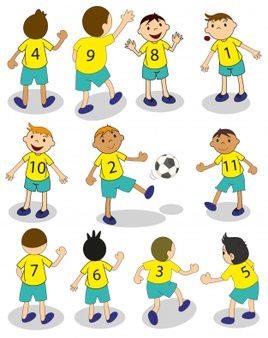
\includegraphics[width=0.5\textwidth]{images/image_003.jpg}
    \end{center}
  \end{columns}
\end{frame}

% Slide 16: The Data - Example 2
\begin{frame}{The Data -- an Example (2)}
  \textbf{The variable:} The shoe sizes of a soccer team with the following observations:

  \begin{center}
    40, 39, 38, 41, 46, 39, 39, 38, 37, 40, 39
  \end{center}
\end{frame}

% Slide 17: Frequency Table
\begin{frame}{Frequency Table}
  \begin{center}
    \small\renewcommand{\arraystretch}{1.2}
    \begin{tabular}{lccccccc}
      \toprule
      Shoe size & 37 & 38 & 39 & 40 & 41 & 46 & Total \\
      \midrule
      Absolute frequency & 1 & 2 & 4 & 2 & 1 & 1 & 11 \\
      Relative frequency (decimal) & $0.0909$ & $0.1818$ & $0.3636$ & $0.1818$ & $0.0909$ & $0.0909$ & 1 \\
      Relative frequency in \% & $9.1\,\%$ & $18.2\,\%$ & $36.4\,\%$ & $18.2\,\%$ & $9.1\,\%$ & $9.1\,\%$ & $100\,\%$ \\
      Relative frequency (fraction) & $\tfrac{1}{11}$ & $\tfrac{2}{11}$ & $\tfrac{4}{11}$ & $\tfrac{2}{11}$ & $\tfrac{1}{11}$ & $\tfrac{1}{11}$ & 1 \\
      Cumulative absolute frequency & 1 & 3 & 7 & 9 & 10 & 11 & \\
      Cumulative rel.\ freq.\ (decimal) & $0.0909$ & $0.2727$ & $0.6364$ & $0.8182$ & $0.9091$ & 1 & \\
      Cumulative rel.\ freq.\ (fraction) & $\tfrac{1}{11}$ & $\tfrac{3}{11}$ & $\tfrac{7}{11}$ & $\tfrac{9}{11}$ & $\tfrac{10}{11}$ & 1 & \\
      \bottomrule
    \end{tabular}
  \end{center}
\end{frame}


% Relative frequencies: percent vs percentage points
\begin{frame}{Comparing Relative Frequencies: Percent vs.\ Percentage Points}
  \textbf{Example:} In a customer survey, the share of 5-star ratings rises
  from $f = 40\,\%$ last year to $f = 50\,\%$ this year.
  \begin{columns}[T]
    \begin{column}{0.48\textwidth}
      \begin{block}{Absolute difference of two shares}
        \centering\smallskip
        $\displaystyle 50\,\% - 40\,\% = \mathbf{10}$ \textbf{percentage points}%
        $\vphantom{\dfrac{50\,\%}{40\,\%}}$\par\smallskip
      \end{block}
    \end{column}
    \begin{column}{0.48\textwidth}
      \begin{block}{Relative change of the share}
        \centering\smallskip
        $\dfrac{50\,\% - 40\,\%}{40\,\%} = 0.25 = \mathbf{25\,\%}$\par\smallskip
      \end{block}
    \end{column}
  \end{columns}
  \vspace{0.3cm}
  \inworten{``The share rose by 10 percentage points'' and ``the share rose by
  25\,\%'' describe the \emph{same} change -- once as a difference, once relative
  to the starting level.}
  \kernaussage{Percentage points = \textbf{absolute} difference of two percentages;
  percent = \textbf{relative} change. The two are often confused in business news!}
\end{frame}

% Quick exercise: frequencies of a nominal variable (adapted from SfÖ Teil 1)
\begin{frame}{Exercise -- Frequencies of a Nominal Variable}
  \begin{block}{Problem statement}
    The online retailer from the exercise on levels of measurement records the payment method
    of $n = 10$ orders (I = invoice, P = PayPal, C = card):
    \[ \text{P,\ C,\ I,\ P,\ P,\ C,\ P,\ I,\ C,\ P} \]
    \begin{enumerate}
      \item[a)] Determine the absolute frequencies $h_j$ and the relative frequencies $f_j$
        (fraction, decimal, \%).
      \item[b)] Which share of the orders is \textbf{not} paid by invoice? How many orders is that?
      \item[c)] Last month, $25\,\%$ of the orders were paid by invoice. By how many percentage
        points and by how many percent has this share changed?
      \item[d)] Does a cumulative relative frequency $F(x)$ make sense here? Give a reason.
    \end{enumerate}
  \end{block}
\end{frame}

\begin{frame}{Solution (1/2) -- Frequencies of a Nominal Variable}
  \begin{block}{Rule}
    $h_j$ = number of values equal to $x_j$; \quad $f_j = h_j / n$; \quad
    checks: $\sum_j h_j = n$ and $\sum_j f_j = 1$.
  \end{block}
  \textbf{a)} Count the $n = 10$ orders (I: 2 times, P: 5 times, C: 3 times); column ``Total'' = check:
  \begin{center}
    \renewcommand{\arraystretch}{1.15}
    \begin{tabular}{lcccc}
      \toprule
      Payment method $x_j$ & Invoice & PayPal & Card & Total \\
      \midrule
      Absolute frequency $h_j$ & $2$ & $5$ & $3$ & $10$ \\
      Relative frequency $f_j$ (fraction) & $\tfrac{2}{10}$ & $\tfrac{5}{10}$ & $\tfrac{3}{10}$ & $1$ \\
      Relative frequency $f_j$ (decimal) & $\mathbf{0.20}$ & $\mathbf{0.50}$ & $\mathbf{0.30}$ & $1$ \\
      Relative frequency in \% & $20\,\%$ & $50\,\%$ & $30\,\%$ & $100\,\%$ \\
      \bottomrule
    \end{tabular}
  \end{center}

  \textbf{b)} ``Not by invoice'' = PayPal or card: \
  $f_{\text{PayPal}} + f_{\text{card}} = 0.50 + 0.30 = \mathbf{0.80}$ \ ($= 1 - f_{\text{invoice}}$),\\
  \hspace*{1.2em}i.e.\ $0.80 \cdot 10 = \mathbf{8}$ orders \ (check: $h_{\text{PayPal}} + h_{\text{card}} = 5 + 3 = 8$).
\end{frame}

\begin{frame}{Solution (2/2) -- Frequencies of a Nominal Variable}
  \textbf{c)} Share paid by invoice: last month $25\,\%$, now $f_{\text{invoice}} = 20\,\%$:
  \begin{itemize}
    \item absolute difference: $20\,\% - 25\,\% = \mathbf{-5}$ \textbf{percentage points}
    \item relative change: $(20\,\% - 25\,\%) / 25\,\% = -0.20 = \mathbf{-20\,\%}$
  \end{itemize}

  \medskip
  \textbf{d)} \textbf{No:} the payment method is \textbf{nominal} -- there is no ordering, so
  ``$x_j \leq x$'' is not defined. A cumulative value ``up to PayPal'' would depend on the
  arbitrary order of the columns:
  \begin{itemize}
    \item order invoice, PayPal, card: \ $0.20 + 0.50 = 0.70$
    \item order card, PayPal, invoice: \ $0.30 + 0.50 = 0.80$
  \end{itemize}
  \begin{alertblock}{Remember}
    $h_j$ and $f_j$ exist for every level of measurement, $F(x)$ only from the
    \textbf{ordinal} level upwards.
  \end{alertblock}
\end{frame}

% Slide: Why Statistics Software?
\begin{frame}{Why Statistics Software?}
  \begin{columns}[c]
    \column{0.6\textwidth}
    \begin{block}{Advantages of Modern Software}
      \begin{itemize}
        \item Complex calculations in seconds
        \item Reproducible analyses through scripts
        \item Professional visualisations
        \item Ability to handle large datasets
      \end{itemize}
    \end{block}
    \vspace{0.8em}
    \textbf{In this course:} We use \textbf{Python} with
    \textbf{Jupyter} notebooks or \textbf{VS Code}

    \column{0.35\textwidth}
    \begin{center}
      \begin{tikzpicture}[node distance=4mm, every node/.style={font=\small}]
        \node[flowboxg, minimum width=3.4cm] (d) {Data};
        \node[flowbox,  minimum width=3.4cm, below=of d] (s) {Python script\\[-1pt]{\scriptsize (\texttt{.py} / \texttt{.ipynb})}};
        \node[flowboxo, minimum width=3.4cm, below=of s] (r) {Tables \& figures};
        \draw[flowarr] (d) -- (s);
        \draw[flowarr] (s) -- (r);
      \end{tikzpicture}\\[0.5em]
      {\small\textcolor{gray}{www.python.org}}
    \end{center}
  \end{columns}
\end{frame}

\begin{frame}{What is Python?}
\begin{itemize}
    \item \textbf{Python} is a programming language for statistics, data analysis and much more.

    \vspace{0.3cm}

    \item Typical application areas:
    \begin{itemize}
        \item Data Science
        \item Statistics
        \item Machine Learning
        \item Scientific research
    \end{itemize}

    \vspace{0.3cm}

    \item Strengths of Python:
    \begin{itemize}
        \item Easy-to-read syntax, huge community, free and open source
        \item Large selection of packages (\texttt{numpy}, \texttt{pandas},
              \texttt{scipy}, \texttt{statsmodels}, \texttt{matplotlib})
        \item Same language from data analysis to machine learning and production
    \end{itemize}

    \vspace{0.3cm}

    \item \textbf{Important:} Python + packages are the \textit{computation engine} (perform calculations).
\end{itemize}
\end{frame}

\begin{frame}{Working Environment: Jupyter and VS Code}
\begin{itemize}
    \item \textbf{Jupyter notebooks} (\texttt{.ipynb}) and \textbf{VS Code}
          are the working environments (IDEs) for Python.

    \vspace{0.3cm}

    \item They provide a user-friendly interface:
    \begin{itemize}
        \item Jupyter: code cells with tables and plots directly below,
              plus text for explanations
        \item VS Code: editor for scripts (\texttt{.py}) and notebooks,
              integrated terminal
        \item Plot windows, variable explorer, package management
    \end{itemize}

    \vspace{0.3cm}

    \item \textbf{Analogy:}
    \begin{itemize}
        \item Python = Engine of a car
        \item Jupyter / VS Code = Dashboard and steering wheel
    \end{itemize}

    \vspace{0.3cm}

    \item \textbf{Important:} Jupyter and VS Code only work if Python is installed.
\end{itemize}
\end{frame}

\begin{frame}[fragile]{Installation (Mac \& Windows)}
\small
\begin{itemize}
    \item \textbf{Step 1: Install Python}
    \begin{itemize}
        \item Recommended: \textbf{Anaconda Distribution}
              (\texttt{https://www.anaconda.com/download}) --
              bundles Python, all packages and Jupyter
        \item Alternative: Python from \texttt{https://www.python.org}, then in a terminal:\\
              \texttt{\footnotesize pip install numpy pandas scipy statsmodels matplotlib jupyter}
    \end{itemize}

    \vspace{0.2cm}

    \item \textbf{Step 2: Choose a working environment}
    \begin{itemize}
        \item Jupyter: start \textbf{JupyterLab} (included in Anaconda) or run \texttt{jupyter lab}
        \item VS Code: \texttt{https://code.visualstudio.com} + extensions
              ``Python'' and ``Jupyter''
    \end{itemize}

    \vspace{0.2cm}

    \item \textbf{Step 3: First test} -- run in a notebook cell; no error message means you are ready:
\end{itemize}
\vspace{-0.2cm}
\begin{lstlisting}[xleftmargin=2.2em]
import numpy, pandas, scipy, statsmodels, matplotlib
print(numpy.__version__, pandas.__version__)
\end{lstlisting}
\end{frame}



% Slide 18: Frequencies with Python
\begin{frame}[fragile]{Frequencies with Python}
\begin{lstlisting}
import pandas as pd

# Soccer team – shoe sizes of the 11 players
data = pd.Series([40, 39, 38, 41, 46, 39, 39, 38, 37, 40, 39])

# Frequency table (absolute frequencies), sorted by shoe size
print(data.value_counts().sort_index())

# Relative frequencies
print(data.value_counts(normalize=True).sort_index())

# Cumulative (relative) frequencies
print(data.value_counts(normalize=True).sort_index().cumsum())
\end{lstlisting}
{\small \textbf{Note:} \texttt{value\_counts()} sorts by frequency;
\texttt{sort\_index()} orders by shoe size (needed for \texttt{cumsum()}).}
\end{frame}

% Slide 19: Column Chart
\begin{frame}{Column Chart}
  \begin{center}
    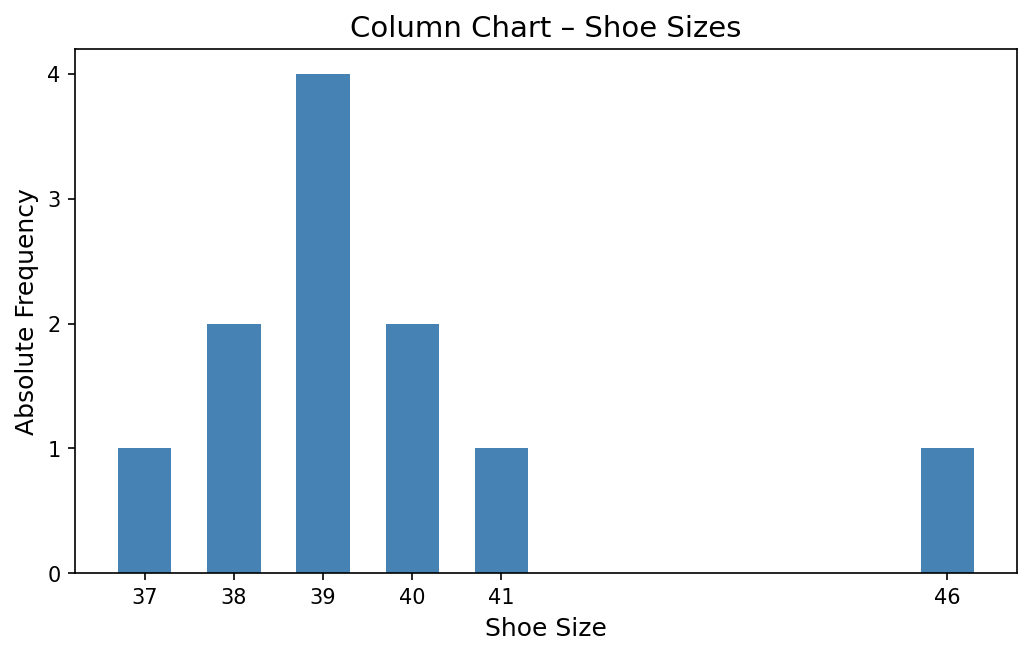
\includegraphics[width=0.8\textwidth,height=0.75\textheight,keepaspectratio]{images/chart_slide_19.png}
  \end{center}
\end{frame}

% Slide 20: Bar Chart
\begin{frame}{Bar Chart}
  \begin{center}
    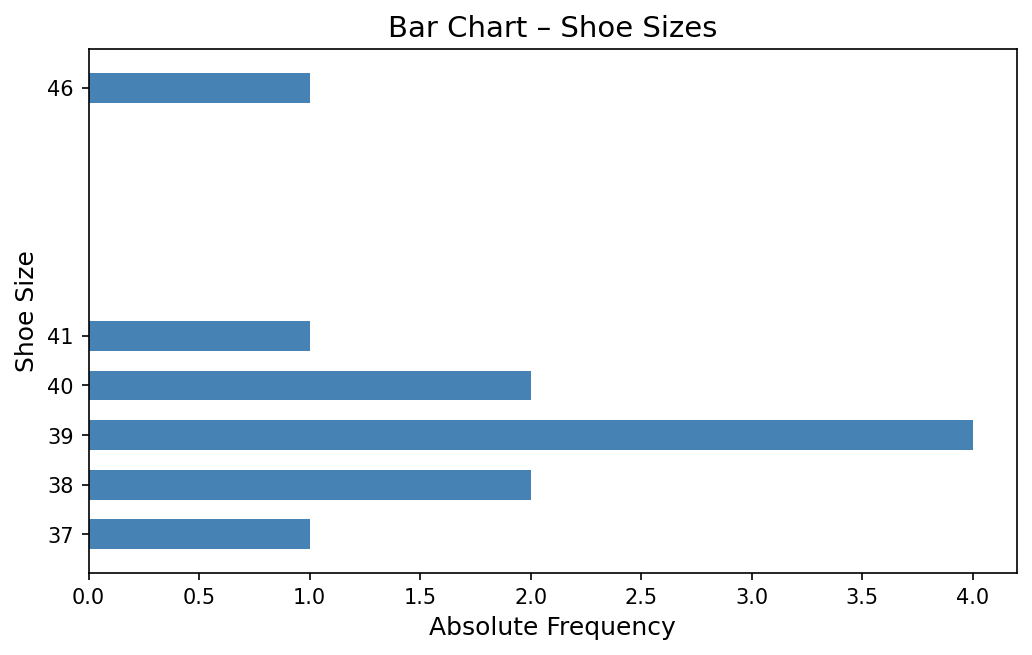
\includegraphics[width=0.8\textwidth,height=0.75\textheight,keepaspectratio]{images/chart_slide_20.png}
  \end{center}
\end{frame}

% Slide 21: Pie Chart
\begin{frame}{Pie Chart}
  \begin{center}
    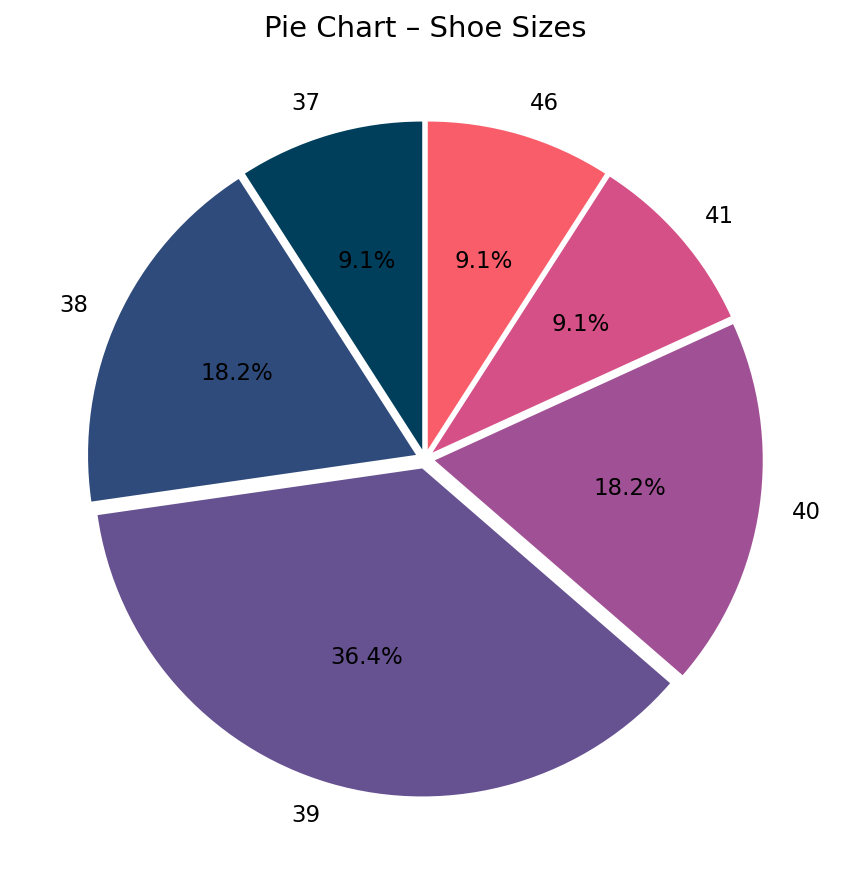
\includegraphics[width=0.8\textwidth,height=0.75\textheight,keepaspectratio]{images/chart_slide_21.png}
  \end{center}
\end{frame}

% Slide 22: Empirical Distribution Function
\begin{frame}{Empirical Distribution Function (Empirical CDF, ECDF)}
  \begin{center}
    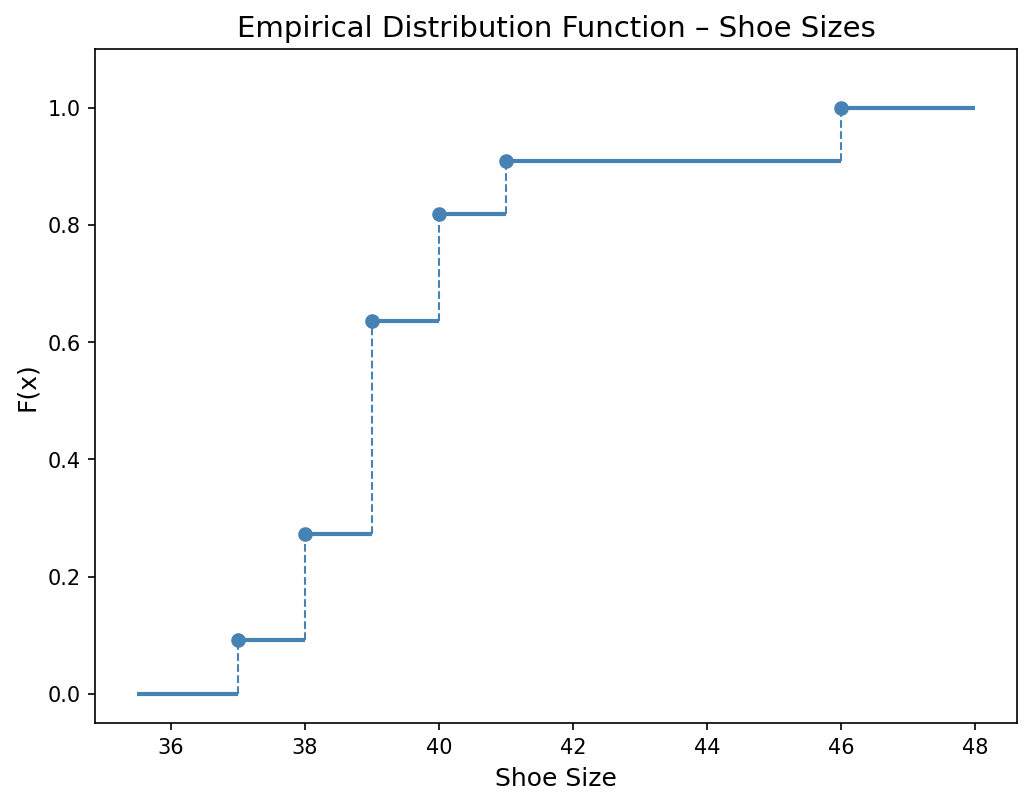
\includegraphics[width=0.8\textwidth,height=0.75\textheight,keepaspectratio]{images/image_004.png}
  \end{center}
\end{frame}

\subsection{Exercises}

\begin{frame}{Exercise -- Frequency Table}
  \begin{block}{Problem statement}
    A café has received $n = 12$ ratings (1 to 5 stars) on a review platform:
    \[ 4,\ 5,\ 3,\ 4,\ 5,\ 5,\ 2,\ 4,\ 5,\ 3,\ 4,\ 5 \]
    \begin{enumerate}
      \item[a)] Set up the frequency table with absolute frequencies $h_j$, relative
        frequencies $f_j$ (as fraction and decimal) and cumulative relative frequencies $F(x_j)$.
      \item[b)] What share of the ratings has \textbf{at most} 3 stars?
      \item[c)] What share of the ratings has \textbf{at least} 4 stars? How many ratings is that?
      \item[d)] Read from the table: which rating is the most frequent one?
      \item[e)] Last year, 30\,\% of the ratings had 5 stars. By how many percentage points
        and by how many percent has this share changed?
    \end{enumerate}
  \end{block}
\end{frame}

\begin{frame}{Solution (1/2) -- Frequency Table}
  \begin{block}{Rule}
    $h_j$ = number of values equal to $x_j$; \ $f_j = h_j / n$; \
    $F(x_j)$ = sum of all $f_l$ with $x_l \leq x_j$.
  \end{block}

  \textbf{a)} Count the $n = 12$ values (check: the $h_j$ add up to $12$, the $f_j$ to $1$):
  \begin{center}
    \renewcommand{\arraystretch}{1.2}
    \begin{tabular}{lccccc}
      \toprule
      Stars $x_j$ & 2 & 3 & 4 & 5 & Total \\
      \midrule
      Absolute frequency $h_j$ & 1 & 2 & 4 & 5 & 12 \\
      Relative frequency $f_j$ (fraction) & $\tfrac{1}{12}$ & $\tfrac{2}{12}$ & $\tfrac{4}{12}$ & $\tfrac{5}{12}$ & 1 \\
      Relative frequency $f_j$ (decimal) & $0.0833$ & $0.1667$ & $0.3333$ & $0.4167$ & 1 \\
      Cumulative rel.\ frequency $F(x_j)$ & $0.0833$ & $\mathbf{0.2500}$ & $0.5833$ & $1$ & \\
      \bottomrule
    \end{tabular}
  \end{center}

  \textbf{b)} ``At most 3 stars'' = cumulative relative frequency at $x = 3$:
  $F(3) = f_1 + f_2 = \tfrac{1}{12} + \tfrac{2}{12} = \tfrac{3}{12} = \mathbf{0.25}$ \ ($x_1 = 2$, $x_2 = 3$) $\to$ a quarter of the ratings.
\end{frame}

\begin{frame}[fragile]{Solution (2/2) -- Frequency Table}
  \textbf{c)} ``At least 4 stars'' = complement of ``at most 3'':
  $1 - F(3) = 1 - 0.25 = \mathbf{0.75}$, i.e.\ $h_3 + h_4 = 4 + 5 = \mathbf{9}$ ratings.

  \textbf{d)} Largest absolute frequency $h_4 = 5$ at $x_4 = 5$ $\to$ the most frequent rating is $\mathbf{5}$ stars.

  \textbf{e)} This year $f_4 = \tfrac{5}{12} = 41.67\,\%$ (last year: $30\,\%$):
  \begin{itemize}
    \item absolute difference: $41.67\,\% - 30\,\% = \mathbf{11.67}$ \textbf{percentage points}
    \item relative change: $(41.67\,\% - 30\,\%) / 30\,\% = 0.389 = \mathbf{38.9\,\%}$
  \end{itemize}
\begin{lstlisting}[keepspaces=true]
stars = pd.Series([4, 5, 3, 4, 5, 5, 2, 4, 5, 3, 4, 5])
print(stars.value_counts().sort_index().tolist())     # [1, 2, 4, 5]
F = stars.value_counts(normalize=True).sort_index().cumsum()
print(F.round(4).tolist())                            # [0.0833, 0.25, 0.5833, 1.0]
print((stars <= 3).mean(), (stars >= 4).sum())        # 0.25 9
\end{lstlisting}
  \begin{alertblock}{Interpretation}
    Three quarters of the guests give 4 or 5 stars; the share of top ratings has grown.
  \end{alertblock}
\end{frame}

% ===== SUBSECTION: MEASURES OF CENTRAL TENDENCY =====
\subsection{Measures of Central Tendency}

\begin{frame}{Measures of Central Tendency}
  \centering\large\textcolor{hsbiblaudunkel}{Measures of Central Tendency -- Means, Median and Quantiles}
\end{frame}

% Slide 24: Measures of Central Tendency
\begin{frame}{Measures of Central Tendency}
  \guidingquestion{Which shoe size is ``typical'' for the soccer team -- and how do we
  summarise eleven values in a single number?}
  \begin{itemize}
    \item Where is the middle?
    \item Where is the centre of gravity of the distribution?
    \item At which value is one quarter of the values reached?
    \item At which value are three quarters of the values reached?
  \end{itemize}
\end{frame}

% Refresher: summation and product sign (needed for the means)
\begin{frame}{Refresher: Summation and Product Signs}
  \textbf{Example data} (first three players): \ $x_1 = 40$, \ $x_2 = 39$, \ $x_3 = 38$
  \begin{columns}[T]
    \begin{column}{0.48\textwidth}
      \begin{block}{Summation sign $\Sigma$}
        \[ \sum_{i=1}^{n} x_i = x_1 + x_2 + \cdots + x_n \]
        Read: ``sum of the $x_i$ for $i$ from $1$ to $n$''\\[3pt]
        Example: $\sum_{i=1}^{3} x_i = 40 + 39 + 38 = 117$
      \end{block}
    \end{column}
    \begin{column}{0.48\textwidth}
      \begin{block}{Product sign $\Pi$}
        \[ \prod_{i=1}^{n} x_i = x_1 \cdot x_2 \cdots x_n \]
        Read: ``product of the $x_i$ for $i$ from $1$ to $n$''\\[3pt]
        Example: $\prod_{i=1}^{3} x_i = 40 \cdot 39 \cdot 38 = 59\,280$
      \end{block}
    \end{column}
  \end{columns}
  \vspace{0.2cm}
  \begin{alertblock}{Common mistake}
    $\sum x_i^2 \neq \bigl(\sum x_i\bigr)^2$, \ e.g.\ $1^2 + 2^2 = 5 \neq (1+2)^2 = 9$:
    first square, then add (as in the variance later)!
  \end{alertblock}
\end{frame}

% Slide 25: Means (1) -- arithmetic and trimmed mean
\begin{frame}{Means (1): Arithmetic Mean and Trimmed Mean}
  \begin{block}{Arithmetic mean}
    Sum of all values divided by $n$:
    \quad $\displaystyle \bar{x} = \frac{1}{n}\sum_{i=1}^{n} x_i$
  \end{block}
  \inworten{the value every unit would have if the total were shared out equally.}

  \smallskip
  \textbf{Advantage:} easy to compute. \quad \textbf{Disadvantage:} sensitive to extreme values (outliers).
  \begin{block}{Trimmed mean $\bar{x}_{\text{trim}}$}
    Choose a share $\alpha$ (e.g.\ $10\,\%$) to cut off at each end: remove the $\lfloor \alpha \cdot n \rfloor$
    smallest and the $\lfloor \alpha \cdot n \rfloor$ largest values ($\lfloor\cdot\rfloor$ = round down),
    then take the arithmetic mean of the rest.
  \end{block}
  \textbf{Example} (shoe sizes, $\alpha = 10\,\%$): $\lfloor 0.1 \cdot 11 \rfloor = 1$ value per end
  $\to$ remove $37$ and $46$:
  \[ \bar{x}_{\text{trim}} = \frac{436 - 37 - 46}{9} = \frac{353}{9} = 39.2222 \]
\end{frame}

% Means (2) -- geometric mean and growth rates
\begin{frame}{Means (2): Geometric Mean -- Averaging Growth Rates}
  \begin{block}{Geometric mean (only for positive values)}
    Product of all values, $n$-th root:
    \quad $\bar{x}_{\text{geo}} = \bigl(\prod_{i=1}^{n} x_i\bigr)^{1/n} = \sqrt[n]{x_1 \cdot x_2 \cdots x_n}$
  \end{block}
  \textbf{Motivation:} revenue grows by $r_1 = +20\,\%$ in year 1 and by $r_2 = -10\,\%$ in year 2.
  Is the average growth $(20\,\% - 10\,\%)/2 = 5\,\%$ per year? \ \textbf{No!}
  \begin{itemize}
    \item Growth rate $r_i$ $\to$ \textbf{growth factor} $1 + r_i$: \ $1.20$ and $0.90$
    \item Factors \textbf{multiply}: $1.20 \cdot 0.90 = 1.08$, i.e.\ $+8\,\%$ in total
    \item Average factor: $\bar{x}_{\text{geo}} = \sqrt{1.08} = 1.0392$ $\to$ $\mathbf{+3.92\,\%}$ per year
    \item Check: $1.0392^2 \approx 1.08$ \checkmark, \ whereas $1.05^2 = 1.1025 \neq 1.08$
  \end{itemize}
  \kernaussage{Average growth rate $= \bar{x}_{\text{geo}}$ of the growth factors $1 + r_i$, minus $1$.
  $\bar{x}_{\text{geo}}$ is the \emph{constant} factor that produces the same total growth.}
\end{frame}

% Slide 26: Median
\begin{frame}{Median}
  \begin{block}{Definition}
    At or below which observation do at least 50\,\% of the values lie?
  \end{block}

  \begin{description}
    \item[Computation:] sort the data; the median is the value at position $\lceil n/2 \rceil$:
      \ $\tilde{x} = x_{(\lceil n/2 \rceil)}$
  \end{description}

  \begin{alertblock}{Note: alternative definition}
    In some textbooks, the median for even $n$ is defined as the average of the two
    middle values (the ``middle value''). In this course, we use the $\lceil n/2 \rceil$ definition.
  \end{alertblock}

  \begin{columns}[T]
    \begin{column}{0.5\textwidth}
      \textbf{Advantages of the $\lceil n/2 \rceil$ definition:}
      \begin{itemize}
        \item The median is always an actual observation
        \item Consistent with the quantile definition:
              Median = 50\,\%-quantile $= x_{(\lceil 0.5 \cdot n \rceil)}$
      \end{itemize}
    \end{column}
    \begin{column}{0.48\textwidth}
      \textbf{Advantages of the median in general:}
      \begin{itemize}
        \item Robust to outliers
        \item Also suitable for ordinal data
      \end{itemize}
    \end{column}
  \end{columns}
\end{frame}

% Slide 27: Mode
\begin{frame}{Mode}
  \begin{block}{Definition}
    The most frequent value in the distribution
  \end{block}

  \begin{itemize}
    \item \textbf{Advantage:} suitable for both ordinal and nominal data
    \item \textbf{Disadvantage:} often not unique
    \item \textbf{Disadvantage:} may not represent the ``centre'' of the distribution
  \end{itemize}
\end{frame}

% Which measure for which level of measurement?
\begin{frame}{Which Measure for Which Level of Measurement?}
  \begin{center}
    \renewcommand{\arraystretch}{1.3}
    \begin{tabular}{lccc}
      \toprule
      \textbf{Level} & \textbf{Mode} & \textbf{Median, quantiles} & \textbf{Arithmetic mean} \\
      \midrule
      Nominal & \checkmark & -- & -- \\
      Ordinal & \checkmark & \checkmark & -- \\
      Metric  & \checkmark & \checkmark & \checkmark \\
      \bottomrule
    \end{tabular}
  \end{center}
  \begin{itemize}
    \item Median and quantiles need a \textbf{ranking}, the mean needs meaningful \textbf{differences}.
    \item The geometric mean needs positive values on a ratio scale (e.g.\ growth factors).
  \end{itemize}
  \begin{exampleblock}{Back to the online retailer (exercise in the Fundamentals)}
    \textbf{Mean} (and median, mode): number of items, order value, delivery time, order date\\
    \textbf{Median} (and mode), no mean: customer rating, customer status\\
    \textbf{Only the mode:} postcode, payment method
  \end{exampleblock}
\end{frame}

% Slide 28: Measures of Central Tendency Example
\begin{frame}{Measures of Central Tendency -- Example}
  \begin{center}
    \begin{tabular}{l*{11}{r}}
      \toprule
      Player & 1 & 2 & 3 & 4 & 5 & 6 & 7 & 8 & 9 & 10 & 11 \\
      \midrule
      Shoe size & 40 & 39 & 38 & 41 & 46 & 39 & 39 & 38 & 37 & 40 & 39 \\
      \bottomrule
    \end{tabular}
  \end{center}

  \begin{center}
    \begin{tabular}{ll}
      \toprule
      \textbf{Measure} & \textbf{Value} \\
      \midrule
      Sum & 436 \\
      Arithmetic mean & 39.6364 \\
      Geometric mean & 39.5755 \\
      Trimmed mean (10\,\% per end) & 39.2222 \\
      Median & 39 \\
      Mode & 39 \\
      \bottomrule
    \end{tabular}
  \end{center}
\end{frame}

% Quick exercise: mean, median, mode, trimmed mean and level of measurement
\begin{frame}{Exercise -- Mean, Median and Mode}
  \begin{block}{Problem statement}
    An electronics shop records the number of laptops sold on $n = 9$ days:
    \[ 4,\ 7,\ 3,\ 5,\ 4,\ 6,\ 4,\ 2,\ 10 \]
    \begin{enumerate}
      \item[a)] Compute the arithmetic mean, the median, the mode and the trimmed mean
        with $\alpha = 20\,\%$.
      \item[b)] On day~9 the shop actually sold $19$ laptops (a large company order), not $10$.
        Which of the four measures change, and to which value?
      \item[c)] $n = 7$ customers rate the service: \ good, very good, fair, good, poor, good,
        very good.\\ Which of the measures may be used for this variable? Determine them.
    \end{enumerate}
  \end{block}
\end{frame}

\begin{frame}{Solution (1/2) -- Mean, Median and Mode}
  \begin{block}{Rule}
    Sort first; \ $\bar{x} = \frac{1}{n}\sum x_i$; \quad median $= x_{(\lceil n/2 \rceil)}$; \quad
    mode = most frequent value;\\ trimmed mean: drop $\lfloor \alpha \cdot n \rfloor$ values at each
    end, then average the rest.
  \end{block}
  \textbf{a)} Sorted data: \ $2,\ 3,\ 4,\ 4,\ 4,\ 5,\ 6,\ 7,\ 10$ \qquad (sum $= 45$)
  \begin{exampleblock}{Calculation}
    \vspace{-0.3cm}
    \begin{align*}
      \bar{x} &= \frac{45}{9} = \mathbf{5}, \qquad
      \tilde{x} = x_{(\lceil 9/2 \rceil)} = x_{(5)} = \mathbf{4}, \qquad
      \text{mode} = \mathbf{4} \ (\text{occurs 3 times}) \\[2pt]
      \bar{x}_{\text{trim}} &= \frac{45 - 2 - 10}{7} = \frac{33}{7} = \mathbf{4.7143}
      \qquad (\lfloor 0.2 \cdot 9 \rfloor = \lfloor 1.8 \rfloor = 1 \text{ value removed per end})
    \end{align*}
  \end{exampleblock}
  \textbf{b)} With $19$ instead of $10$ the sum grows by $9$ to $54$ $\to$
  $\bar{x} = 54 / 9 = \mathbf{6}$ (up by $1$). The order is unchanged ($19$ is still the
  largest value) $\to$ median $= \mathbf{4}$, mode $= \mathbf{4}$ and
  $\bar{x}_{\text{trim}} = (54 - 2 - 19) / 7 = \mathbf{4.7143}$ stay the same.
\end{frame}

\begin{frame}{Solution (2/2) -- Mean, Median and Mode}
  \textbf{c)} The service rating is \textbf{ordinal}: the categories have a ranking
  (poor $<$ fair $<$ good $<$ very good), but the distances between them are not meaningful.
  \begin{itemize}
    \item Sorted: \ poor, fair, good, good, good, very good, very good
    \item Median: $x_{(\lceil 7/2 \rceil)} = x_{(4)} = \textbf{good}$
    \item Mode: \textbf{good} (3 of the 7 ratings)
    \item Arithmetic (and trimmed) mean: \textbf{not meaningful} -- ``(good + poor)\,/\,2'' is not
      defined, and the step from poor to fair need not equal the step from good to very good.
  \end{itemize}
  \begin{alertblock}{Interpretation}
    A single extreme day moves the mean ($5 \to 6$), but not the median, the mode or the trimmed
    mean: these are \textbf{robust} to outliers. For ordinal data, use the median and the mode.
  \end{alertblock}
\end{frame}

% Mean from a frequency table
\begin{frame}{Arithmetic Mean from a Frequency Table}
  \textbf{Idea:} if the data are given as a frequency table, each value $x_j$ enters the sum $h_j$ times.
  \begin{block}{Rule}
    \[ \bar{x} = \frac{1}{n}\sum_{j=1}^{k} h_j \cdot x_j = \sum_{j=1}^{k} f_j \cdot x_j
       \qquad (k = \text{number of distinct values}) \]
  \end{block}
  \begin{center}
    \renewcommand{\arraystretch}{1.2}
    \begin{tabular}{lccccccc}
      \toprule
      Shoe size $x_j$ & 37 & 38 & 39 & 40 & 41 & 46 & Total \\
      \midrule
      $h_j$ & 1 & 2 & 4 & 2 & 1 & 1 & 11 \\
      $h_j \cdot x_j$ & 37 & 76 & 156 & 80 & 41 & 46 & 436 \\
      \bottomrule
    \end{tabular}
  \end{center}
  $\bar{x} = \frac{436}{11} = \mathbf{39.6364}$ -- the same result as from the raw data.

  \medskip
  \inworten{a \emph{weighted} mean: every value counts as often as it occurs; the weights
  are the relative frequencies $f_j$.}
\end{frame}

% Slide 29: Measures of Central Tendency with Python
\begin{frame}[fragile]{Measures of Central Tendency with Python (1)}
\begin{lstlisting}
import numpy as np
from scipy import stats

# Sum
print(data.sum())                  # 436

# Arithmetic mean
print(data.mean())                 # 39.6364

# Geometric mean
# Step 1: Calculate the product of all values
product = np.prod(data)
# Step 2: Determine the number of observations
n = len(data)
# Step 3: Take the n-th root
gmean = product ** (1 / n)         # 39.5755
print(stats.gmean(data))           # same result in one step
\end{lstlisting}
\end{frame}

% Slide 29: Measures of Central Tendency with Python
\begin{frame}[fragile]{Measures of Central Tendency with Python (2)}
\begin{lstlisting}
# Trimmed mean: 10% of the values are removed at EACH end
print(stats.trim_mean(data, 0.10))  # 39.2222

# Median
print(np.median(data))              # 39.0

# Mode (all most frequent values, as a list)
print(data.mode().tolist())         # [39]

# Mean from a frequency table: weighted mean
print(np.average([37, 38, 39, 40, 41, 46], weights=[1, 2, 4, 2, 1, 1]))  # 39.6364
\end{lstlisting}
\begin{alertblock}{Note: NumPy's median definition}
  For even $n$, \texttt{np.median()} averages the two middle values -- the
  course definition $x_{(\lceil n/2 \rceil)}$ is obtained with
  \texttt{np.quantile(data, 0.5, method="inverted\_cdf")}.
\end{alertblock}
\end{frame}

% Slide 30: Quantiles
\begin{frame}{Quantiles}
  \textbf{First, the values must be sorted!}

  \begin{description}
    \item[1st quartile:] At or below which value do at least 25\,\% of the values lie?
    \item[2nd quartile:] = Median (at or below which value do at least 50\,\% of the values lie?)
    \item[3rd quartile:] At or below which value do at least 75\,\% of the values lie?
    \item[Arbitrary $p$-quantile:] At or below which value do at least $p \cdot 100\,\%$ of the values lie?
  \end{description}
\end{frame}

% Slide 31: Quantile Computation
\begin{frame}{Quantiles -- Computation}
  \begin{block}{Rule (course definition)}
    \[ x_p = x_{(\lceil n \cdot p \rceil)} \]
    Compute $n \cdot p$ and round \textbf{up} to the next integer: this is the position in the
    sorted data. If $n \cdot p$ is already an integer, it stays as it is.
  \end{block}
  \inworten{count $\lceil n \cdot p \rceil$ values from the bottom of the sorted list -- at least
  $p \cdot 100\,\%$ of the observations lie at or below this value.}

  \vspace{0.4cm}
  \textbf{Example} 80\,\%-quantile ($n = 11$): $n \cdot 0.8 = 11 \cdot 0.8 = 8.8$, round up to
  position 9 $\to$ $x_{0.8} = x_{(9)} = 40$.

  \vspace{0.2cm}
  \textbf{Example} $n = 10$, $p = 0.2$: $n \cdot p = 2$ is already an integer $\to$ position 2.
\end{frame}

% Slide 32: Quantile Computation - Example
\begin{frame}{Quantiles -- Computation Example}
  \begin{center}
    \normalsize
    \begin{tabular}{lcccc}
      \toprule
      Quantile & $p$ & $n \cdot p$ & Position & Value \\
      \midrule
      1st quartile & 0.25 & 2.75 & 3 & 38 \\
      2nd quartile & 0.50 & 5.50 & 6 & 39 \\
      3rd quartile & 0.75 & 8.25 & 9 & 40 \\
      17\,\%-quantile & 0.17 & 1.87 & 2 & 38 \\
      80\,\%-quantile & 0.80 & 8.80 & 9 & 40 \\
      5\,\%-quantile & 0.05 & 0.55 & 1 & 37 \\
      \bottomrule
    \end{tabular}
  \end{center}
\end{frame}

% Slide 33: Quantile Worked Example
\begin{frame}{Quantiles -- Worked Example}
  Sorted data: 37, 38, 38, 39, 39, 39, 39, 40, 40, 41, 46

  \vspace{0.5cm}

  \begin{align*}
    \text{Median} &= x_{(\lceil 0.5 \cdot 11 \rceil)} = x_{(6)} = 39 \\
    Q_1 &= x_{(\lceil 0.25 \cdot 11 \rceil)} = x_{(3)} = 38 \\
    Q_3 &= x_{(\lceil 0.75 \cdot 11 \rceil)} = x_{(9)} = 40
  \end{align*}
\end{frame}

% Quick exercise: quantiles by hand (course definition)
\begin{frame}{Exercise -- Quantiles of Hotline Waiting Times}
  \begin{block}{Problem statement}
    A customer hotline measures the waiting time (in minutes, rounded) of $n = 12$ calls:
    \[ 3,\ 1,\ 5,\ 2,\ 6,\ 4,\ 2,\ 8,\ 3,\ 4,\ 2,\ 5 \]
    \begin{enumerate}
      \item[a)] Sort the data.
      \item[b)] Determine the $10\,\%$-quantile, $Q_1$, the median, $Q_3$ and the $90\,\%$-quantile.
      \item[c)] The hotline wants to promise: ``At least $90\,\%$ of our callers wait at most
        $x$ minutes.'' What is the smallest $x$ supported by the data?
      \item[d)] A colleague reports a median of $3.5$ minutes. How did they obtain this value,
        and what is the median according to the course definition?
    \end{enumerate}
  \end{block}
\end{frame}

\begin{frame}{Solution (1/2) -- Quantiles of Hotline Waiting Times}
  \begin{block}{Rule}
    $x_p = x_{(\lceil n \cdot p \rceil)}$: round $n \cdot p$ \textbf{up} (an integer stays as it is);
    take the value at this position.
  \end{block}
  \textbf{a)} Sorted data ($x_{(1)}, \ldots, x_{(12)}$): \quad
  $1,\ 2,\ 2,\ 2,\ 3,\ 3,\ 4,\ 4,\ 5,\ 5,\ 6,\ 8$

  \medskip
  \textbf{b)} Quantiles for $n = 12$:
  \begin{center}
    \renewcommand{\arraystretch}{1.1}
    \begin{tabular}{lcccc}
      \toprule
      Quantile & $p$ & $n \cdot p$ & Position & Value \\
      \midrule
      $10\,\%$-quantile & $0.10$ & $1.2$ & $2$ & $x_{(2)} = \mathbf{2}$ \\
      $Q_1$ & $0.25$ & $3.0$ & $3$ & $x_{(3)} = \mathbf{2}$ \\
      Median & $0.50$ & $6.0$ & $6$ & $x_{(6)} = \mathbf{3}$ \\
      $Q_3$ & $0.75$ & $9.0$ & $9$ & $x_{(9)} = \mathbf{5}$ \\
      $90\,\%$-quantile & $0.90$ & $10.8$ & $11$ & $x_{(11)} = \mathbf{6}$ \\
      \bottomrule
    \end{tabular}
  \end{center}
  {\small Note: $x_{0.1} = Q_1 = 2$ because of ties (three calls of exactly $2$ minutes) -- only the position counts.}
\end{frame}

\begin{frame}{Solution (2/2) -- Quantiles of Hotline Waiting Times}
  \textbf{c)} The promise asks for the $90\,\%$-quantile: \ $x_{0.9} = x_{(11)} = \mathbf{6}$ minutes.
  \begin{itemize}
    \item Check with the cumulative relative frequency: \ $F(6) = \tfrac{11}{12} = 0.9167 \geq 0.9$ \checkmark
    \item $5$ minutes are not enough: \ $F(5) = \tfrac{10}{12} = 0.8333 < 0.9$
  \end{itemize}

  \medskip
  \textbf{d)} The colleague averaged the two middle values $x_{(6)} = 3$ and $x_{(7)} = 4$:
  $(3 + 4) / 2 = 3.5$ -- the alternative textbook definition for even $n$.
  The course definition gives \ $\tilde{x} = x_{(\lceil 12/2 \rceil)} = x_{(6)} = \mathbf{3}$ minutes.
  \begin{alertblock}{Interpretation}
    At least half of the callers wait at most $3$ minutes and at least $90\,\%$ at most $6$ minutes
    -- only the single caller with $8$ minutes waits longer.
  \end{alertblock}
\end{frame}

\begin{comment}
% Slide 34: Quantile Computation - Alternative
\begin{frame}{Quantiles -- Computation (alternative)}
  For the $p$-quantile: round up $n \cdot p$, position in sorted values

  \vspace{0.5cm}

  \begin{block}{Alternative}
    The quantiles can be read from the empirical distribution function, both from the data table describing the function and from the graphical representation.
  \end{block}
\end{frame}

\begin{frame}{Reading Quantiles from the Empirical Distribution Function}

\small

\textbf{Key idea:}
The empirical distribution function \(F_n(x)\) indicates \emph{what proportion of observations is less than or equal to \(x\)}.

\vspace{0.8em}

\[
F_n(x) = \frac{\#\{x_i \leq x\}}{n}
\]

\vspace{0.8em}

\textbf{Quantiles reverse this question:}
A \(p\)-quantile is the value \(x_p\) at which at least the proportion \(p\) of the data is reached.

\vspace{0.8em}

\[
x_p = \min \{x \in \mathbb{R} \mid F_n(x) \geq p \}
\]

\vspace{0.8em}

\textbf{Reading from the empirical distribution function:}
\begin{itemize}
    \item \textbf{From the table:} Find the smallest value \(x\) for which \(F_n(x) \geq p\).
    \item \textbf{From the graph:} Go on the y-axis to proportion \(p\), then horizontally to the step function, and finally vertically down to the x-axis.
\end{itemize}

\vspace{0.8em}

\textbf{Example:}
The 50\%-quantile (median) is the smallest value \(x\) for which \(F_n(x) \geq 0.5\).

\end{frame}

% Slide 35: Empirical Distribution Function
\begin{frame}{Empirical Distribution Function}
  \begin{center}
    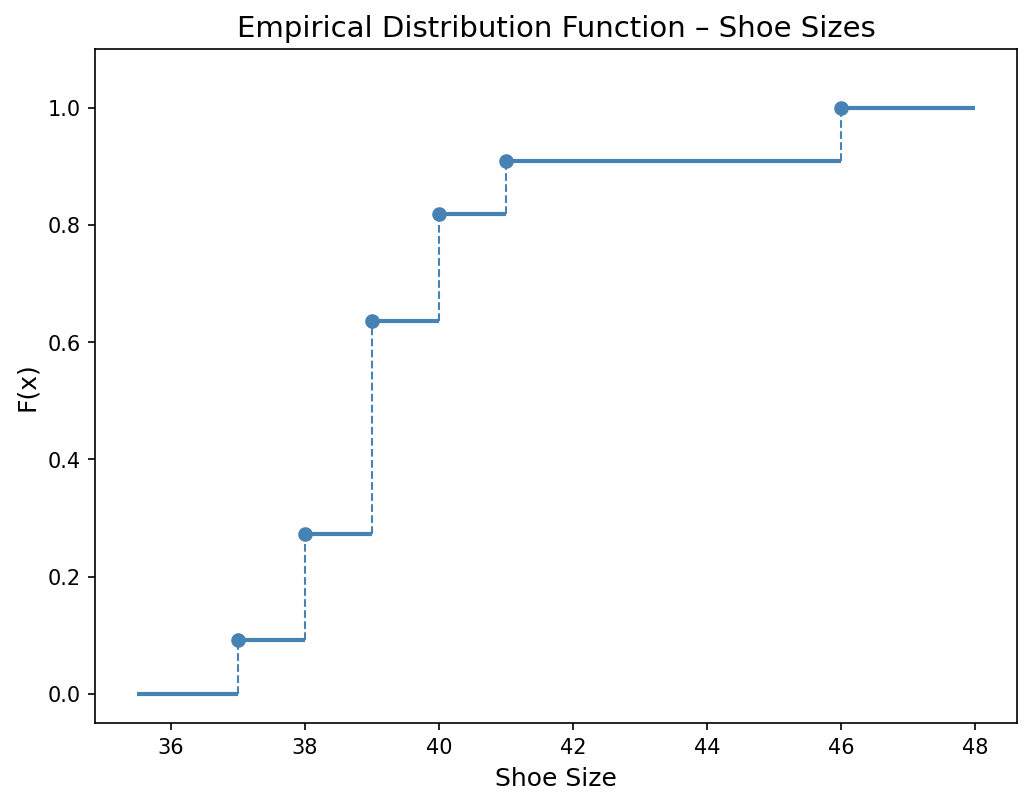
\includegraphics[width=0.8\textwidth,height=0.75\textheight,keepaspectratio]{images/image_004.png}
  \end{center}
\end{frame}

\end{comment}


% Slide 36: Quantiles with Python
\begin{frame}[fragile]{Quantiles with Python}
\begin{lstlisting}
# Course definition x_(ceil(n*p)): method="inverted_cdf"
# All standard quantiles at once (0, 25, 50, 75, 100 %)
p = [0, 0.25, 0.50, 0.75, 1]
print(np.quantile(data, p, method="inverted_cdf"))   # [37 38 39 40 46]

# 1st quartile (25%-quantile)
print(np.quantile(data, 0.25, method="inverted_cdf"))  # 38

# 80%-quantile
print(np.quantile(data, 0.80, method="inverted_cdf"))  # 40
\end{lstlisting}
\begin{alertblock}{Pitfall: the default method interpolates}
  \texttt{np.quantile(data, 0.25)} and \texttt{data.quantile(0.25)} use
  linear interpolation and return $38.5$ -- always pass
  \texttt{method="inverted\_cdf"} to get the course definition.
\end{alertblock}
\end{frame}

\subsection{Exercises}

\begin{frame}{Exercise -- Measures of Central Tendency and Quantiles}
  \begin{block}{Problem statement}
    Annual salaries (in thousand euros) of the $n = 10$ employees of a department,
    including the head of department:
    \[ 34,\ 42,\ 28,\ 120,\ 36,\ 31,\ 45,\ 34,\ 50,\ 39 \]
    \begin{enumerate}
      \item[a)] Sort the data and compute the arithmetic mean, the median and the mode.
      \item[b)] Compute the trimmed mean (remove $10\,\%$ of the values at each end).
      \item[c)] Determine $Q_1$, $Q_3$ and the $20\,\%$- and $90\,\%$-quantiles.
      \item[d)] Which measure best describes the ``typical'' salary in the department? Give reasons.
    \end{enumerate}
  \end{block}
\end{frame}

\begin{frame}{Solution (1/4) -- Measures of Central Tendency and Quantiles}
  \begin{block}{Rule}
    Sort first; \ $\bar{x} = \frac{1}{n}\sum x_i$; \quad median $= x_{(\lceil n/2 \rceil)}$; \quad mode = most frequent value.
  \end{block}

  \textbf{a)} Sorted data ($x_{(1)}, \ldots, x_{(10)}$): \quad $28,\ 31,\ 34,\ 34,\ 36,\ 39,\ 42,\ 45,\ 50,\ 120$
  \begin{exampleblock}{Calculation}
    \vspace{-0.3cm}
    \begin{align*}
      \bar{x} &= \frac{28 + 31 + 34 + 34 + 36 + 39 + 42 + 45 + 50 + 120}{10} = \frac{459}{10} = \mathbf{45.9} \\[2pt]
      \tilde{x} &= x_{(\lceil 0.5 \cdot 10 \rceil)} = x_{(5)} = \mathbf{36} \\[2pt]
      \text{Mode} &= \mathbf{34} \quad (\text{the only value that occurs twice})
    \end{align*}
  \end{exampleblock}
  The arithmetic mean ($45.9$) lies far above the median ($36$): $8$ of the $10$ employees
  earn less than the average.
\end{frame}

\begin{frame}{Solution (2/4) -- Measures of Central Tendency and Quantiles}
  \textbf{b)} Trimmed mean: $\lfloor 0.1 \cdot 10 \rfloor = 1$ value per end $\to$ remove $28$ and $120$,
  average the rest:
  \[ \bar{x}_{\text{trim}} = \frac{31 + 34 + 34 + 36 + 39 + 42 + 45 + 50}{8} = \frac{311}{8} = \mathbf{38.875} \]

  \textbf{c)} Rule: position $= \lceil n \cdot p \rceil$ in the sorted data; if $n \cdot p$ is already
  an integer, it is not rounded up.
  \begin{center}
    \renewcommand{\arraystretch}{1.1}
    \begin{tabular}{lcccc}
      \toprule
      Quantile & $p$ & $n \cdot p$ & Position & Value \\
      \midrule
      $20\,\%$-quantile & $0.20$ & $2.0$ & $2$ & $x_{(2)} = \mathbf{31}$ \\
      $Q_1$ & $0.25$ & $2.5$ & $3$ & $x_{(3)} = \mathbf{34}$ \\
      $Q_3$ & $0.75$ & $7.5$ & $8$ & $x_{(8)} = \mathbf{45}$ \\
      $90\,\%$-quantile & $0.90$ & $9.0$ & $9$ & $x_{(9)} = \mathbf{50}$ \\
      \bottomrule
    \end{tabular}
  \end{center}

  {\small Note: $x_{(3)} = x_{(4)} = 34$ -- ties (equal values) do not change the rule; only the position counts.}
\end{frame}

\begin{frame}{Solution (3/4) -- Measures of Central Tendency and Quantiles}
  \textbf{d)} The salary of the head of department ($120$) is an outlier and pulls the mean up to
  $45.9$ -- a salary hardly anyone in the department earns. The \textbf{median ($36$)} and the
  trimmed mean ($38.9$) are robust to the outlier and describe the typical salary better.
  \begin{center}
    \begin{tikzpicture}[x=0.118cm, y=1cm]
      \draw[->, thick, hsbigrau!70!black] (25,0) -- (127,0)
        node[right, font=\footnotesize, text=black, align=left] {thousand\\ euros};
      \foreach \t in {30,40,...,120}
        \draw[hsbigrau!70!black] (\t,0.07) -- (\t,-0.07) node[below, font=\footnotesize, text=black] {\t};
      \foreach \v in {28,31,34,36,39,42,45,50,120}
        \fill[hsbiblau] (\v,0.2) circle (2.6pt);
      \fill[hsbiblau] (34,0.42) circle (2.6pt);
      \draw[hsbigruen, very thick] (36,0) -- (36,0.9)
        node[above left=-1mm, font=\footnotesize, text=hsbigruen] {median $36$};
      \draw[hsbiorange, very thick] (38.875,0) -- (38.875,1.35)
        node[above right=-1mm, font=\footnotesize, text=hsbiorange!80!black] {trimmed mean $38.875$};
      \draw[hsbirot, very thick] (45.9,0) -- (45.9,0.9)
        node[above right=-1mm, font=\footnotesize, text=hsbirot] {mean $45.9$};
      \node[above=2mm, font=\footnotesize, text=hsbiblaudunkel] at (120,0.2) {head of department};
    \end{tikzpicture}
  \end{center}
  \kernaussage{For skewed data with outliers (salaries, wealth, sales) always report the median
  \textbf{and} the mean -- the gap between them reveals the skewness.}
\end{frame}

\begin{frame}[fragile]{Solution (4/4) -- Measures of Central Tendency and Quantiles}
\begin{lstlisting}
# Python check; course quantiles need method="inverted_cdf"
salary = np.array([34, 42, 28, 120, 36, 31, 45, 34, 50, 39])
print(np.sort(salary))
print(salary.mean(), stats.trim_mean(salary, 0.10))
print(pd.Series(salary).mode().tolist())
print(np.quantile(salary, 0.5, method="inverted_cdf"), np.median(salary))
print(np.quantile(salary, [0.2, 0.25, 0.75, 0.9], method="inverted_cdf"))
\end{lstlisting}
\begin{lstlisting}[style=Pyout]
[ 28  31  34  34  36  39  42  45  50 120]
45.9 38.875
[34]
36 37.5
[31 34 45 50]
\end{lstlisting}
  \begin{alertblock}{Pitfall: even $n$}
    \texttt{np.median()} returns $37.5$, the average of $x_{(5)} = 36$ and $x_{(6)} = 39$.
    The course median is $x_{(\lceil 10/2 \rceil)} = x_{(5)} = 36$.
  \end{alertblock}
\end{frame}

\begin{frame}{Exercise -- Geometric Mean}
  \begin{block}{Problem statement}
    The revenue of a start-up was exactly $200$ thousand euros in year~0. In the following
    three years it changed by
    \[ +10\,\%, \qquad -5\,\%, \qquad +20\,\%. \]
    \begin{enumerate}
      \item[a)] What is the revenue after three years?
      \item[b)] Compute the arithmetic mean of the three growth rates. Which revenue after three
        years would you obtain if revenue had grown by this mean every year?
      \item[c)] Compute the average annual growth rate via the geometric mean of the growth
        factors and check the result.
      \item[d)] Why does the arithmetic mean in b) give a wrong result?
    \end{enumerate}
  \end{block}
\end{frame}

\begin{frame}{Solution (1/2) -- Geometric Mean}
  \begin{block}{Rule}
    Growth rate $r_i$ $\to$ growth factor $1 + r_i$. Several periods: \textbf{multiply} the factors.
  \end{block}

  \textbf{a)} Growth factors: $1.10$; \ $0.95$; \ $1.20$
  \[ \text{Revenue}_3 = 200 \cdot 1.10 \cdot 0.95 \cdot 1.20 = 200 \cdot 1.254 = \mathbf{250.8} \text{ thousand euros} \]

  \textbf{b)} Arithmetic mean of the rates:
  \[ \bar{r} = \frac{0.10 - 0.05 + 0.20}{3} = \frac{0.25}{3} = 0.0833 = \mathbf{8.33\,\%} \]
  With this mean: $200 \cdot 1.0833^3 = 200 \cdot 1.2714 = \mathbf{254.3}$ thousand euros
  $\neq 250.8$ $\to$ \textbf{too high!}
\end{frame}

\begin{frame}[fragile]{Solution (2/2) -- Geometric Mean}
  \textbf{c)} Geometric mean of the growth factors:
  \[ \bar{x}_{\text{geo}} = \left(1.10 \cdot 0.95 \cdot 1.20\right)^{1/3} = 1.254^{1/3} = \mathbf{1.0784}
     \quad\Rightarrow\quad \bar{r}_{\text{geo}} = 1.0784 - 1 = \mathbf{7.84\,\%} \]
  Check: $200 \cdot 1.0784^3 \approx 200 \cdot 1.254 = 250.8$ thousand euros \checkmark

  \textbf{d)} Growth acts \textbf{multiplicatively}: the $+20\,\%$ applies to a different base than
  the $+10\,\%$. The arithmetic mean of the rates is never smaller than the geometric one and
  thus overstates the growth.
\begin{lstlisting}
factors = np.array([1.10, 0.95, 1.20])
print(200 * np.prod(factors))       # 250.8
print(factors.mean() - 1)           # 0.0833  (arithmetic: wrong)
print(stats.gmean(factors) - 1)     # 0.0784  (geometric: correct)
\end{lstlisting}
  \kernaussage{Average growth rates, returns, price increases: use the
  \textbf{geometric mean of the growth factors}.}
\end{frame}

% ===== SUBSECTION: MEASURES OF DISPERSION =====
\subsection{Measures of Dispersion}

\begin{frame}{Measures of Dispersion}
  \centering\large\textcolor{hsbiblaudunkel}{Measures of Dispersion -- Range, Interquartile Range,\\[0.3em]
  Variance, Standard Deviation,\\[0.3em]
  Coefficient of Variation, Normalised Coefficient of Variation}
\end{frame}

% Slide 38: Measures of Dispersion - Why?
\begin{frame}{Measures of Dispersion -- Why?}
  \textit{Example: Shoe sizes of two women's rowing fours (without coxswain)}

  \vspace{0.3cm}

  \begin{center}
    \begin{tabular}{lcc}
      \toprule
      & \textbf{Four A} & \textbf{Four B} \\
      \midrule
      Data & 34, 37, 40, 41 & 36, 37, 39, 40 \\
      Mean & 38 & 38 \\
      Median & 37 & 37 \\
      \bottomrule
    \end{tabular}
  \end{center}

  \vspace{0.5cm}

  \begin{block}{Question}
    The mean and median are identical. Does that mean the data sets are equivalent?
  \end{block}
\end{frame}

% Slide 39b: Measures of Dispersion Visualisation
\begin{frame}{Measures of Dispersion -- Visualisation}
  \begin{center}
    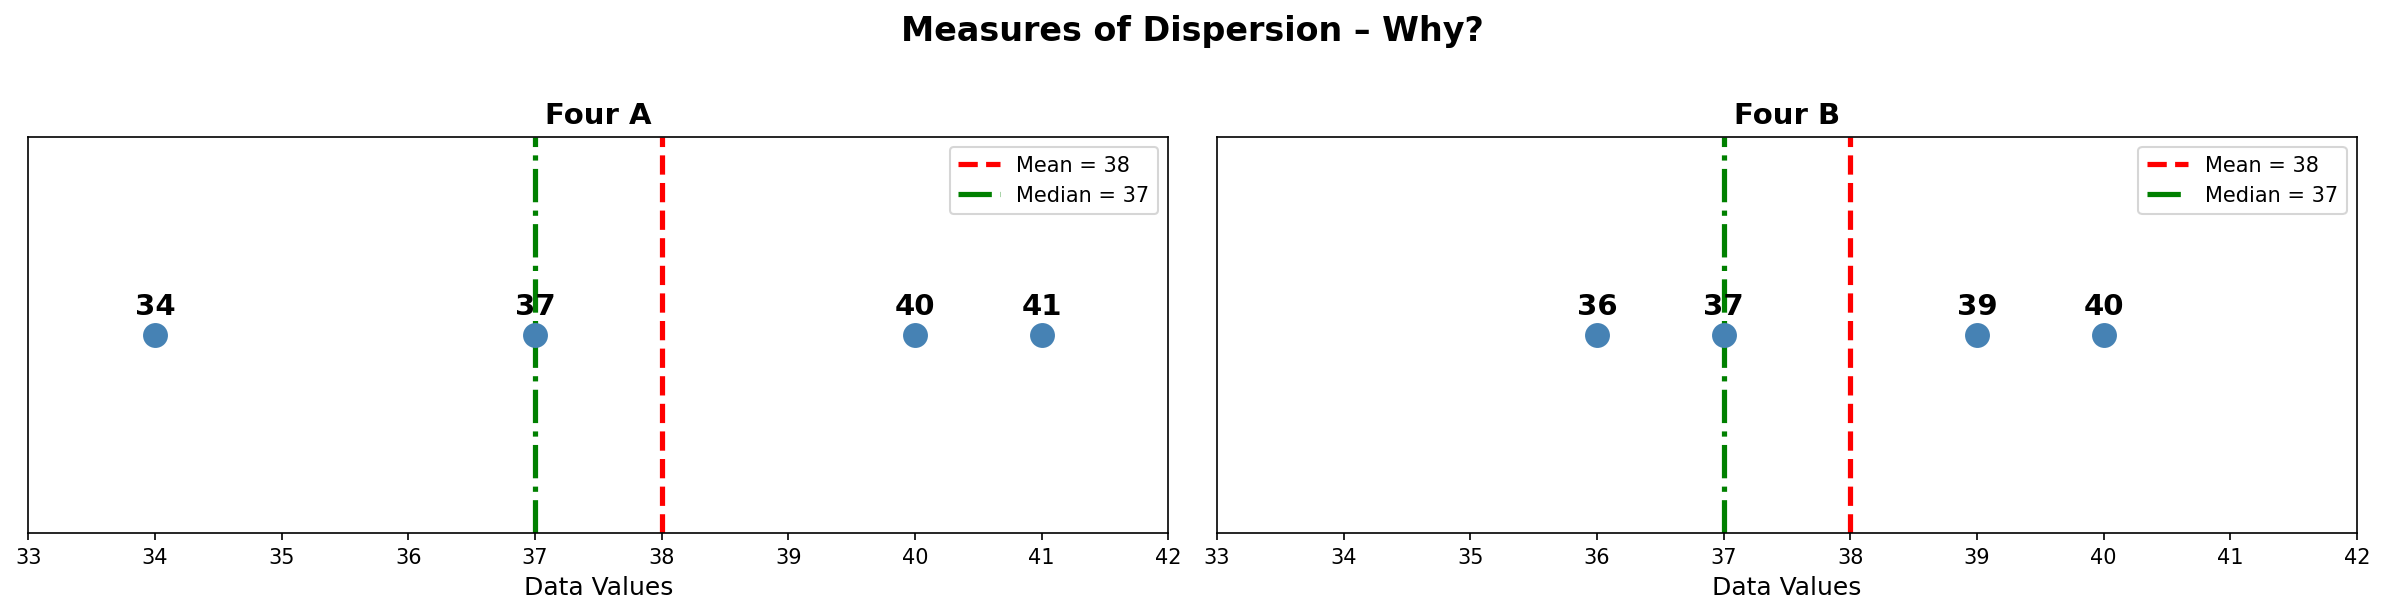
\includegraphics[width=0.9\textwidth,height=0.9\textheight,keepaspectratio]{images/streuung_viz.png}
  \end{center}
  \vspace{-0.3cm}
  \begin{itemize}
    \item Mean and median are identical -- but the \textbf{dispersion} differs considerably
    \item Four A: Data farther from the mean $\to$ greater dispersion
    \item Four B: Data closely concentrated around the mean $\to$ less dispersion
  \end{itemize}
\end{frame}

% Range and interquartile range
\begin{frame}{Range and Interquartile Range}
  \begin{block}{Definitions}
    \textbf{Range:} \quad $R = x_{(n)} - x_{(1)}$ \ (largest minus smallest value)\\[3pt]
    \textbf{Interquartile range:} \quad $\text{IQR} = Q_3 - Q_1 = x_{0.75} - x_{0.25}$
  \end{block}
  \inworten{$R$ is the width of the whole data set, the IQR the width of its middle 50\,\%.}

  \textbf{Example} (soccer team, sorted): \ 37, 38, \textbf{38}, 39, 39, 39, 39, 40, \textbf{40}, 41, 46
  \begin{itemize}
    \item $R = 46 - 37 = \mathbf{9}$, \quad $\text{IQR} = x_{(9)} - x_{(3)} = 40 - 38 = \mathbf{2}$
    \item Rowing fours: $R_A = 41 - 34 = 7 > R_B = 40 - 36 = 4$ \ and \
          $\text{IQR}_A = 40 - 34 = 6 > \text{IQR}_B = 39 - 36 = 3$
  \end{itemize}
  \begin{alertblock}{Range vs.\ IQR}
    $R$ depends only on the two most extreme values: the player with size 46 alone makes
    $R = 9$. The IQR ignores the outer 25\,\% on each side and is \textbf{robust} to outliers.
  \end{alertblock}
\end{frame}

\begin{frame}{Sample Variance}
  \begin{block}{Definition}
    Mean squared deviation from the mean (corrected with $n-1$):
    \[ s^2 = \frac{1}{n-1}\sum_{i=1}^{n}(x_i - \bar{x})^2 \qquad 0 \leq s^2 < \infty \]
  \end{block}
  \inworten{roughly the average squared distance of the values from their mean.}
  \begin{itemize}
    \item \textbf{Why square?} -- The deviations from the mean always cancel out exactly,
      $\sum_{i=1}^{n}(x_i - \bar{x}) = 0$. Squaring makes every deviation count positively.
    \item \textbf{Why divide by $n-1$ only?} -- Because using the mean leaves only $n-1$ degrees of freedom:
      if the mean and $n-1$ values are known, the $n$-th value can be computed.
    \item The dimension has changed, e.g.\ cm becomes cm$^2$.
    \item Comparison requires the same units. With different $n$, the precision of the estimates may differ.
  \end{itemize}
\end{frame}


\begin{frame}{Sample Variance -- Worked Example}
  \begin{center}
    \begin{tabular}{lcc}
      \toprule
      & \textbf{Four A} & \textbf{Four B} \\
      \midrule
      Data & 34, 37, 40, 41 & 36, 37, 39, 40 \\
      Mean $\bar{x}$ & 38 & 38 \\
      Deviations $x_i - \bar{x}$ & $-4,\ -1,\ +2,\ +3$ & $-2,\ -1,\ +1,\ +2$ \\
      \bottomrule
    \end{tabular}
  \end{center}

  {\small Check: the deviations sum to $0$ in both cases.}

  \begin{exampleblock}{Calculation}
    \begin{align*}
      s^2_A &= \frac{1}{4-1}\bigl[(34-38)^2 + (37-38)^2 + (40-38)^2 + (41-38)^2\bigr] = \frac{30}{3} = 10 \\[4pt]
      s^2_B &= \frac{1}{4-1}\bigl[(36-38)^2 + (37-38)^2 + (39-38)^2 + (40-38)^2\bigr] = \frac{10}{3} \approx 3.33
    \end{align*}
  \end{exampleblock}
\end{frame}

\begin{frame}{Standard Deviation}
  \begin{block}{Definition}
    The standard deviation is the square root of the variance:
    \[ s = +\sqrt{s^2} \qquad 0 \leq s < \infty \]
  \end{block}

  \begin{itemize}
    \item By taking the square root, the measure of dispersion is again in the \textbf{dimension of the original values}
    \item If $s = 0$: no dispersion -- all values are equal and equal the mean
    \item Same unit as the original values, therefore \textbf{more intuitive} than the sample variance
    \item Comparison requires the same units. With different $n$, the precision of the estimates may differ.
  \end{itemize}

\end{frame}

\begin{frame}{Standard Deviation -- Worked Example}

  \begin{exampleblock}{Calculation}
    \begin{align*}
      s_A &= +\sqrt{s^2_A} = +\sqrt{10} = 3.1623 \\[4pt]
      s_B &= +\sqrt{s^2_B} = +\sqrt{3.\overline{3}} = 1.8257
    \end{align*}
  \end{exampleblock}

  \vspace{0.1cm}

  \begin{alertblock}{Interpretation}
    The values of Four A scatter around the mean with a standard deviation of about
    $3.16$ shoe sizes, the values of Four B only with about $1.83$.

    $\to$ The dispersion is now expressed in the \textbf{same unit} as the original data.
  \end{alertblock}
\end{frame}

% Quick exercise: variance and standard deviation by hand (adapted from SfÖ Teil 1)
\begin{frame}{Exercise -- Variance and Standard Deviation}
  \begin{block}{Problem statement}
    The online retailer compares two parcel services. Delivery times (in days) of $n = 5$ orders each:
    \begin{center}
      \renewcommand{\arraystretch}{1.15}
      \begin{tabular}{lccccc}
        \toprule
        Order $i$ & 1 & 2 & 3 & 4 & 5 \\
        \midrule
        Parcel service A & 2 & 5 & 1 & 3 & 4 \\
        Parcel service B & 4 & 3 & 5 & 4 & 4 \\
        \bottomrule
      \end{tabular}
    \end{center}
    \begin{enumerate}
      \item[a)] Compute the mean $\bar{x}$ and the range $R$ for both services.
      \item[b)] Compute the sample variance $s^2$ and the standard deviation $s$ (with units).
      \item[c)] Which service delivers faster on average, which more reliably? Give reasons.
    \end{enumerate}
  \end{block}
\end{frame}

\begin{frame}{Solution (1/2) -- Variance and Standard Deviation}
  \begin{block}{Rule}
    Deviations from the mean, square them, add them up, divide by $n - 1 = 4$: \
    $s^2 = \frac{1}{n-1}\sum_{i=1}^{n}(x_i - \bar{x})^2$; \quad $s = +\sqrt{s^2}$.
  \end{block}
  \textbf{a)} Means: \ $\bar{x}_A = \frac{2 + 5 + 1 + 3 + 4}{5} = \frac{15}{5} = \mathbf{3}$ days, \quad
  $\bar{x}_B = \frac{4 + 3 + 5 + 4 + 4}{5} = \frac{20}{5} = \mathbf{4}$ days\\[2pt]
  \hspace*{1.2em}Ranges: \ $R_A = 5 - 1 = \mathbf{4}$ days, \quad $R_B = 5 - 3 = \mathbf{2}$ days
  \begin{center}
    \renewcommand{\arraystretch}{1.05}
    \begin{tabular}{lcccccc}
      \toprule
      Order $i$ & 1 & 2 & 3 & 4 & 5 & Total \\
      \midrule
      A: $x_i - 3$ & $-1$ & $2$ & $-2$ & $0$ & $1$ & $0$ \\
      A: $(x_i - 3)^2$ & $1$ & $4$ & $4$ & $0$ & $1$ & $10$ \\
      \midrule
      B: $x_i - 4$ & $0$ & $-1$ & $1$ & $0$ & $0$ & $0$ \\
      B: $(x_i - 4)^2$ & $0$ & $1$ & $1$ & $0$ & $0$ & $2$ \\
      \bottomrule
    \end{tabular}
  \end{center}
  Check: the deviations sum to $0$ for both services \checkmark
\end{frame}

\begin{frame}{Solution (2/2) -- Variance and Standard Deviation}
  \textbf{b)} Divide the sums of squares by $n - 1 = 4$, then take the square root:
  \begin{align*}
    s^2_A &= \frac{10}{4} = \mathbf{2.5} \text{ days}^2, & s_A &= \sqrt{2.5} = \mathbf{1.5811} \text{ days} \\[2pt]
    s^2_B &= \frac{2}{4} = \mathbf{0.5} \text{ days}^2, & s_B &= \sqrt{0.5} = \mathbf{0.7071} \text{ days}
  \end{align*}
  \textbf{c)} Comparison:
  \begin{itemize}
    \item \textbf{Faster on average:} service \textbf{A} ($\bar{x}_A = 3$ days vs.\ $\bar{x}_B = 4$ days)
    \item \textbf{More reliable:} service \textbf{B} ($s_B = 0.71$ vs.\ $s_A = 1.58$ days; $R_B = 2$ vs.\
      $R_A = 4$ days): its delivery times stay close to the mean, those of A range from $1$ to $5$ days
  \end{itemize}
  \begin{alertblock}{Interpretation}
    To promise a fixed delivery date, choose B; to be fast on average, choose A.
    The standard deviation can be read directly in \textbf{days}, the variance (in days$^2$) cannot.
  \end{alertblock}
\end{frame}

% Variance from a frequency table
\begin{frame}{Variance from a Frequency Table}
  \begin{block}{Rule: as for the mean, every squared deviation enters the sum $h_j$ times}
    \[ s^2 = \frac{1}{n-1}\sum_{j=1}^{k} h_j \cdot (x_j - \bar{x})^2 \]
  \end{block}
  \begin{center}
    \small\renewcommand{\arraystretch}{1.1}
    \begin{tabular}{lccccccc}
      \toprule
      Soccer team: $x_j$ & 37 & 38 & 39 & 40 & 41 & 46 & Total \\
      \midrule
      $h_j$ & 1 & 2 & 4 & 2 & 1 & 1 & 11 \\
      $x_j - \bar{x}$ \ ($\bar{x} = 39.6364$) & $-2.6364$ & $-1.6364$ & $-0.6364$ & $0.3636$ & $1.3636$ & $6.3636$ & \\
      $h_j \cdot (x_j - \bar{x})^2$ & $6.9504$ & $5.3554$ & $1.6198$ & $0.2645$ & $1.8595$ & $40.4959$ & $56.5455$ \\
      \bottomrule
    \end{tabular}
  \end{center}
  \centerline{$s^2 = 56.5455 / 10 = \mathbf{5.6545}, \qquad s = \sqrt{5.6545} = \mathbf{2.3779}$}
  \vspace{0.15cm}
  \textcolor{hsbirot}{\textbf{Observation:}} the single value 46 contributes $40.50$ of $56.55$
  ($72\,\%$) to the sum of squares $\to$ $s^2$ and $s$ react strongly to outliers.
\end{frame}

\begin{frame}{Coefficient of Variation}
  \begin{block}{Definition}
    The coefficient of variation is a \textbf{relative} measure of dispersion:
    \[ v = \frac{s}{\bar{x}} \qquad \text{for data with } x_i > 0 \text{ for all } i \text{ (hence } \bar{x} > 0) \]
  \end{block}

  \begin{itemize}
    \item \textbf{Relative} means: independent of the scale (order of magnitude)
    \item The values must all be positive (ratio scale with a natural zero)
      \begin{itemize}
        \item Mathematically: $\bar{x} > 0$, since otherwise division by zero or a negative $v$
        \item Substantively: $\bar{x}$ must reflect a meaningful \textbf{level} of the data
        \item With mixed signs, $\bar{x} \approx 0$ is possible -- then $v$ becomes extremely large, even though the dispersion is not unusual
        \item Example: $-10, -5, +5, +11 \Rightarrow \bar{x} = 0.25$, $v$ loses its interpretive value
      \end{itemize}
    \item Typical applications: incomes, weights, prices
    \item However: with very different sample sizes, the precision of the estimates differs, so comparisons should be interpreted with caution
  \end{itemize}
\end{frame}


\begin{frame}{Coefficient of Variation -- Worked Example}

  \begin{exampleblock}{Calculation}
    \begin{align*}
      v_A &= \frac{s_A}{\bar{x}_A} = \frac{3.1623}{38} = 0.0832 \\[4pt]
      v_B &= \frac{s_B}{\bar{x}_B} = \frac{1.8257}{38} = 0.0480
    \end{align*}
  \end{exampleblock}

  \vspace{0.2cm}

  \begin{alertblock}{Interpretation}
    The standard deviation of Four A amounts to about $8.3\,\%$ of its mean, that of Four B
    to only about $4.8\,\%$.

    $\to$ As a relative measure, $v$ allows comparison of dispersions \textbf{regardless of the scale} of the data.
  \end{alertblock}
\end{frame}



\begin{frame}{Normalised Coefficient of Variation}
  \begin{block}{Definition}
    The normalised coefficient of variation is a relative measure of dispersion
    \textbf{normalised} to the interval $[0, 1]$:
    \[ v^* = \frac{s}{\bar{x}} \cdot \frac{1}{\sqrt{n}} = \frac{v}{\sqrt{n}} \qquad 0 \leq v^* \leq 1 \]
  \end{block}

  \begin{itemize}
    \item Same prerequisites as for the coefficient of variation $v$
    \item \textbf{Background:} for non-negative data, $v$ is at most $\sqrt{n}$ (extreme case: all
      values but one are $0$). Dividing by $\sqrt{n}$ therefore puts $v$ on a scale from $0$ to $1$.
    \item \textbf{Advantage over $v$:} $v^* = 0$ means no dispersion, $v^* = 1$ the maximum possible
      dispersion $\to$ one can judge whether the relative dispersion is small or large
      \textbf{in absolute terms}
    \item \textbf{Caution:} $v^*$ is \textbf{not} suitable for comparing samples of different size:
      with the same dispersion, $v^*$ gets smaller just because $n$ is larger ($\propto 1/\sqrt{n}$)
  \end{itemize}
\end{frame}

\begin{frame}{Normalised Coefficient of Variation -- Worked Example}

  \begin{exampleblock}{Calculation}
    \begin{align*}
      v^*_A &= \frac{v_A}{\sqrt{n}} = \frac{0.0832}{\sqrt{4}} = \frac{0.0832}{2} = 0.0416 \\[4pt]
      v^*_B &= \frac{v_B}{\sqrt{n}} = \frac{0.0480}{\sqrt{4}} = \frac{0.0480}{2} = 0.0240
    \end{align*}
  \end{exampleblock}

  \vspace{0.2cm}

  \begin{alertblock}{Interpretation}
    On the scale from $0$ to $1$ both values are close to $0$ $\to$ the relative dispersion is
    very low in both fours; the sizes in Four A vary relatively more than in Four B.

    $\to$ Since both fours have the same $n = 4$, normalising does not change the comparison:
    $v^*_A / v^*_B = v_A / v_B$. With different $n$, a comparison via $v^*$ would not be meaningful.
  \end{alertblock}
\end{frame}


% Slide 44: Overview Measures of Dispersion
\begin{frame}{Overview of Measures of Dispersion}
  \begin{center}
    \normalsize
    \begin{tabular}{lcc}
      \toprule
      & \textbf{Four A} & \textbf{Four B} \\
      \midrule
      Mean & 38 & 38 \\
      Median & 37 & 37 \\
      Range & 7 & 4 \\
      Interquartile range & 6 & 3 \\
      Sample variance & 10 & 3.3333 \\
      Standard deviation & 3.1623 & 1.8257 \\
      Coefficient of variation & 0.0832 & 0.0480 \\
      Normalised coefficient of variation & 0.0416 & 0.0240 \\
      \bottomrule
    \end{tabular}
  \end{center}
\end{frame}

% Slide 45: Measures of Dispersion with Python
\begin{frame}[fragile]{Measures of Dispersion with Python}
\begin{lstlisting}
four_a = np.array([34, 37, 40, 41])
# Range and interquartile range (course quantiles)
print(np.ptp(four_a))                                   # 7
q1, q3 = np.quantile(four_a, [0.25, 0.75], method="inverted_cdf")
print(q3 - q1)                                          # 6
# Sample variance (ddof=1: divide by n-1) and standard deviation
print(np.var(four_a, ddof=1), np.std(four_a, ddof=1))   # 10.0 3.1623
# Coefficient of variation and normalised coefficient of variation
v = np.std(four_a, ddof=1) / np.mean(four_a)            # 0.0832
vstar = v / np.sqrt(len(four_a))                        # 0.0416
\end{lstlisting}
\begin{alertblock}{Pitfall: NumPy divides by $n$ by default}
  \texttt{np.var(four\_a)} uses \texttt{ddof=0} and returns $7.5$ instead of
  $s^2 = 10$ -- always pass \texttt{ddof=1}. pandas' \texttt{.var()} and
  \texttt{.std()} already use \texttt{ddof=1}.
\end{alertblock}
\end{frame}

\subsection{Exercises}

\begin{frame}{Exercise -- Which Measure of Dispersion for Which Comparison?}
  \begin{block}{Problem statement}
    Which measures of dispersion ($s^2$, $s$, $v$, $v^*$) are suitable for comparing
    \begin{enumerate}
      \item the shoe sizes of the rowing four and the rowing eight?
      \item the shoe sizes of the women's four and the men's four?
      \item the shoe sizes of the women's four and the women's four with coxswain?
      \item the shoe sizes of the women's four and the men's eight?
    \end{enumerate}
  \end{block}
\end{frame}

\begin{frame}{Hint -- Which Measure of Dispersion?}
  \begin{block}{When is which measure suitable?}
    The sample size affects $s^2$, $s$ and $v$ only through the \textbf{precision of the estimate},
    not the measure itself -- an eight with the same dispersion as a four has (apart from random
    fluctuations) the same $s$ and the same $v$. Only $v^*$ gets smaller just because $n$ is larger.
  \end{block}

  \vspace{0.2cm}

  \begin{center}
    \renewcommand{\arraystretch}{1.3}
    \begin{tabular}{lcc}
      \toprule
      \textbf{Measure of dispersion} & \textbf{Scale (order of magnitude)} & \textbf{Sample size $n$} \\
      \midrule
      Sample variance $s^2$              & dependent   & measure independent of $n$ \\
      Standard deviation $s$             & dependent   & measure independent of $n$ \\
      Coefficient of variation $v$       & independent & measure independent of $n$ \\
      Norm.\ coeff.\ of variation $v^*$  & independent & decreases with $n$ ($\propto 1/\sqrt{n}$) \\
      \bottomrule
    \end{tabular}
  \end{center}
\end{frame}

\begin{frame}{Solution (1/3) -- Which Measure of Dispersion?}

  \textbf{1. Four vs.\ eight} (same unit, same scale, \textbf{different $n$})
  \begin{itemize}
    \item $s^2$, $s$, $v$: \textbf{yes} -- the measures do not depend on $n$; the different $n$
      ($4$ vs.\ $8$) only affects the precision of the estimate
    \item $v^*$: \textbf{no} -- the eight would get a smaller $v^*$ just because $\sqrt{8} > \sqrt{4}$,
      even with the same dispersion
  \end{itemize}

  \vspace{0.2cm}

  \textbf{2. Women's four vs.\ men's four} (same unit, \textbf{different scale}, same $n$)
  \begin{itemize}
    \item $s^2$, $s$: less suitable, since men's shoe sizes are systematically larger
    \item $v$: \textbf{yes} -- not affected by the scale
    \item $v^*$: \textbf{yes} -- with equal $n$ only a rescaling of $v$
  \end{itemize}

\end{frame}

\begin{frame}{Solution (2/3) -- Which Measure of Dispersion?}

  \textbf{3. Women's four vs.\ women's four with coxswain} (same unit, same scale, \textbf{different $n$})
  \begin{itemize}
    \item $s^2$, $s$, $v$: \textbf{yes} -- measures independent of $n$; the different $n$
      ($4$ vs.\ $5$) only affects the precision of the estimate
    \item $v^*$: \textbf{no} -- divided by $\sqrt{5}$ instead of $\sqrt{4}$, the comparison is distorted
  \end{itemize}

  \vspace{0.2cm}

  \textbf{4. Women's four vs.\ men's eight} (\textbf{different scale} and \textbf{different $n$})
  \begin{itemize}
    \item $s^2$, $s$: less suitable, the scale differs
    \item $v$: \textbf{yes} -- not affected by the scale and independent of $n$
    \item $v^*$: \textbf{no} -- the different $n$ distorts the comparison
  \end{itemize}
\end{frame}


\begin{frame}{Solution (3/3) -- Which Measure of Dispersion?}
  \begin{enumerate}
    \item The shoe sizes of the rowing four and the rowing eight.
    \item The shoe sizes of the women's four and the men's four.
    \item The shoe sizes of the women's four and the women's four with coxswain.
    \item The shoe sizes of the women's four and the men's eight.
  \end{enumerate}

  \vspace{0.6em}
  \begin{center}
    \renewcommand{\arraystretch}{1.3}
    \begin{tabular}{lcccc}
      \toprule
       & \textbf{1.} & \textbf{2.} & \textbf{3.} & \textbf{4.} \\
      \midrule
      Sample variance                     & yes & no  & yes & no \\
      Standard deviation                  & yes & no  & yes & no \\
      Coefficient of variation            & yes & yes & yes & yes \\
      Normalised coefficient of variation & no  & yes & no  & no \\
      \bottomrule
    \end{tabular}
  \end{center}
\end{frame}

% Exercise: handball team
\begin{frame}{Exercise -- Measures of Dispersion of the Handball Team}
  \begin{block}{Problem statement}
    Shoe sizes of the handball team ($n = 13$): \
    $40,\ 39,\ 38,\ 41,\ 46,\ 39,\ 39,\ 38,\ 37,\ 40,\ 39,\ 40,\ 42$

    \medskip
    Calculate the following measures:
    \begin{center}
      \renewcommand{\arraystretch}{1.2}
      \begin{tabular}{llc}
        \toprule
        \textbf{Measure} & \textbf{Formula} & \textbf{Value} \\
        \midrule
        Mean $\bar{x}$ & $\frac{1}{n}\sum_{i=1}^{n} x_i$ & ? \\
        Sample variance $s^2$ & $\frac{1}{n-1}\sum_{i=1}^{n}(x_i - \bar{x})^2$ & ? \\
        Standard deviation $s$ & $+\sqrt{s^2}$ & ? \\
        Coefficient of variation $v$ & $s / \bar{x}$ & ? \\
        Norm.\ coeff.\ of variation $v^*$ & $v / \sqrt{n}$ & ? \\
        \bottomrule
      \end{tabular}
    \end{center}
  \end{block}
\end{frame}

\begin{frame}{Solution -- Measures of Dispersion of the Handball Team}
  \textbf{Intermediate values:} \ $\sum x_i = 518$, \quad $\sum (x_i - \bar{x})^2 = 61.6923$
  \begin{center}
    \renewcommand{\arraystretch}{1.15}
    \begin{tabular}{lll}
      \toprule
      \textbf{Measure} & \textbf{Calculation} & \textbf{Value} \\
      \midrule
      Mean $\bar{x}$ & $518 / 13$ & $\mathbf{39.8462}$ \\[2pt]
      Sample variance $s^2$ & $61.6923 / 12$ & $\mathbf{5.1410}$ \\[2pt]
      Standard deviation $s$ & $\sqrt{5.1410}$ & $\mathbf{2.2674}$ \\[2pt]
      Coefficient of variation $v$ & $2.2674 / 39.8462$ & $\mathbf{0.0569}$ \\[2pt]
      Norm.\ coeff.\ of variation $v^*$ & $0.0569 / \sqrt{13}$ & $\mathbf{0.0158}$ \\
      \bottomrule
    \end{tabular}
  \end{center}
  \begin{alertblock}{Interpretation}
    Soccer team: $s = 2.3779$, $v = 2.3779 / 39.6364 = 0.0600$ $\to$ the shoe sizes of both
    teams vary similarly. Their $v^*$ ($0.0158$ vs.\ $0.0181$) must \textbf{not} be compared: $n$ differs
    ($13$ vs.\ $11$).
  \end{alertblock}
\end{frame}

% Exercise: two branches
\begin{frame}{Exercise -- Comparing the Dispersion of Two Branches}
  \begin{block}{Problem statement}
    Monthly revenues (thousand euros) of two bakery branches over the last $n = 6$ months:
    \begin{center}
      \renewcommand{\arraystretch}{1.05}
      \begin{tabular}{lcccccc}
        \toprule
        Month & 1 & 2 & 3 & 4 & 5 & 6 \\
        \midrule
        City branch  & 120 & 130 & 125 & 135 & 115 & 125 \\
        Rural branch & 20  & 24  & 22  & 26  & 18  & 22  \\
        \bottomrule
      \end{tabular}
    \end{center}
    \begin{enumerate}
      \item[a)] Compute the mean $\bar{x}$ and the sample variance $s^2$ for both branches.
      \item[b)] Compute the standard deviation $s$.
      \item[c)] Compute the coefficient of variation $v$ and the normalised coefficient of variation $v^*$.
      \item[d)] Which branch has the stronger revenue fluctuations? Which measure is suitable
        for this comparison, and why?
    \end{enumerate}
  \end{block}
\end{frame}

\begin{frame}{Solution (1/3) -- Comparing the Dispersion of Two Branches}
  \begin{block}{Rule}
    $s^2 = \frac{1}{n-1}\sum (x_i - \bar{x})^2$: square the deviations from the mean, add them up,
    divide by $n - 1 = 5$.
  \end{block}
  \textbf{a)} Means: $\bar{x}_{\text{city}} = \frac{750}{6} = \mathbf{125}$, \quad
  $\bar{x}_{\text{rural}} = \frac{132}{6} = \mathbf{22}$ \quad (check: the deviations sum to $0$)
  \begin{center}
    \renewcommand{\arraystretch}{1.1}
    \begin{tabular}{lccccccc}
      \toprule
      Month $i$ & 1 & 2 & 3 & 4 & 5 & 6 & Total \\
      \midrule
      City: $x_i - 125$ & $-5$ & $5$ & $0$ & $10$ & $-10$ & $0$ & $0$ \\
      City: $(x_i - 125)^2$ & $25$ & $25$ & $0$ & $100$ & $100$ & $0$ & $250$ \\
      \midrule
      Rural: $x_i - 22$ & $-2$ & $2$ & $0$ & $4$ & $-4$ & $0$ & $0$ \\
      Rural: $(x_i - 22)^2$ & $4$ & $4$ & $0$ & $16$ & $16$ & $0$ & $40$ \\
      \bottomrule
    \end{tabular}
  \end{center}
  \[ s^2_{\text{city}} = \frac{250}{5} = \mathbf{50}, \qquad s^2_{\text{rural}} = \frac{40}{5} = \mathbf{8} \]
\end{frame}

\begin{frame}{Solution (2/3) -- Comparing the Dispersion of Two Branches}
  \textbf{b)} Standard deviation $s = +\sqrt{s^2}$:
  \[ s_{\text{city}} = \sqrt{50} = \mathbf{7.0711}, \qquad s_{\text{rural}} = \sqrt{8} = \mathbf{2.8284}
     \quad \text{(both in thousand euros)} \]

  \textbf{c)} Coefficient of variation $v = s / \bar{x}$ and normalised coefficient of variation
  $v^* = v / \sqrt{n}$ with $\sqrt{6} = 2.4495$:
  \begin{align*}
    v_{\text{city}}  &= \frac{7.0711}{125} = \mathbf{0.0566} & v^*_{\text{city}}  &= \frac{0.0566}{2.4495} = \mathbf{0.0231} \\[4pt]
    v_{\text{rural}} &= \frac{2.8284}{22}  = \mathbf{0.1286} & v^*_{\text{rural}} &= \frac{0.1286}{2.4495} = \mathbf{0.0525}
  \end{align*}

  \begin{alertblock}{Observation}
    In absolute terms the city branch fluctuates more ($s = 7.07 > 2.83$), relative to the revenue
    level the rural branch does ($v = 12.9\,\% > 5.7\,\%$). Both $v^*$ are close to $0$ on the
    scale from $0$ to $1$ -- and since $n$ is equal, $v^*$ gives the same ranking as $v$.
  \end{alertblock}
\end{frame}

\begin{frame}[fragile]{Solution (3/3) -- Comparing the Dispersion of Two Branches}
  \textbf{d)} The branches operate on a \textbf{different scale} ($\bar{x} = 125$ vs.\ $22$), so the
  \textbf{relative} measure $v$ is suitable: $v_{\text{rural}} = 0.1286 > v_{\text{city}} = 0.0566$
  $\Rightarrow$ \textbf{the rural branch has the stronger (relative) revenue fluctuations.}
\begin{lstlisting}
city  = np.array([120, 130, 125, 135, 115, 125])
rural = np.array([20, 24, 22, 26, 18, 22])
for x in (city, rural):
    s = x.std(ddof=1)
    print(x.mean(), x.var(ddof=1), round(s, 4), round(s / x.mean(), 4))
\end{lstlisting}
\begin{lstlisting}[style=Pyout]
125.0 50.0 7.0711 0.0566
22.0 8.0 2.8284 0.1286
\end{lstlisting}
  \begin{alertblock}{Interpretation}
    $s = 7.07$ at a level of $125$ weighs less than $s = 2.83$ at $22$: the rural branch fluctuates
    by almost $13\,\%$ of its level, the city branch by less than $6\,\%$ -- harder to plan for.
  \end{alertblock}
\end{frame}

% ===== SUBSECTION: EXAM-STYLE EXERCISE (adapted from mock exam 4, task 1) =====
\subsection{Exam-Style Exercise}

\begin{frame}{Exam-Style Exercise -- Books per Order}
  \begin{block}{Problem statement}
    An online bookshop analyses the number of books per order for $n = 25$ orders:

    \smallskip
    \centerline{\renewcommand{\arraystretch}{1.1}%
      \begin{tabular}{lccccc}
        \toprule
        Books per order $x_j$ & 1 & 2 & 3 & 4 & 5 \\
        Number of orders $h_j$ & 3 & 5 & 9 & 5 & 3 \\
        \bottomrule
      \end{tabular}}
    \begin{enumerate}\setlength{\itemsep}{0pt}
      \item[a)] Complete the frequency table with $f_j$, $H_j$ and $F(x_j)$.
      \item[b)] Which share of the orders contains at most 2 books? Which share at least 4 books?
      \item[c)] Determine the mode, the median, $Q_1$, $Q_3$ (use $H_j$) and the IQR.
      \item[d)] Level of measurement of ``number of books''? Why is the mean meaningful here --
        unlike for star ratings?
      \item[e)] Compute the arithmetic mean from the frequency table.
      \item[f)] Compute $s^2$, $s$ and $v$ from the frequency table.
      \item[g)] Compare mean, median and mode: what do they say about the shape of the distribution?
    \end{enumerate}
  \end{block}
\end{frame}

\begin{frame}{Solution (1/4) -- Books per Order}
  \begin{block}{Rule}
    $f_j = h_j / n$; \ $H_j$ and $F(x_j)$: add up the $h_j$ or the $f_j$ from the left; \
    ``at least 4'' $= 1 - F(3)$.
  \end{block}
  \textbf{a)} Frequency table ($n = 25$; check: $H_5 = 25$, $F(5) = 1$):
  \begin{center}
    \renewcommand{\arraystretch}{1.2}
    \begin{tabular}{lcccccc}
      \toprule
      Books $x_j$ & 1 & 2 & 3 & 4 & 5 & Total \\
      \midrule
      $h_j$ & 3 & 5 & 9 & 5 & 3 & 25 \\
      $f_j = h_j / 25$ & $0.12$ & $0.20$ & $0.36$ & $0.20$ & $0.12$ & $1$ \\
      $H_j$ & 3 & 8 & 17 & 22 & 25 & \\
      $F(x_j)$ & $0.12$ & $\mathbf{0.32}$ & $0.68$ & $0.88$ & $1$ & \\
      \bottomrule
    \end{tabular}
  \end{center}
  \textbf{b)} At most 2 books: $F(2) = \frac{3 + 5}{25} = \mathbf{0.32}$ \ (32\,\% of the orders).\\[2pt]
  At least 4 books: $1 - F(3) = 1 - 0.68 = \mathbf{0.32}$ \ ($= \frac{5 + 3}{25}$, also 32\,\%).
\end{frame}

\begin{frame}{Solution (2/4) -- Books per Order}
  \textbf{c)} Mode: largest frequency $h_3 = 9$ $\to$ $\mathbf{3}$ books.

  \smallskip
  Quantiles: position $m = \lceil n \cdot p \rceil$; the value at position $m$ is the first $x_j$ with
  $H_j \geq m$.
  \begin{center}
    \renewcommand{\arraystretch}{1.15}
    \begin{tabular}{lcccl}
      \toprule
      & $p$ & $n \cdot p$ & Position & Value \\
      \midrule
      $Q_1$ & $0.25$ & $6.25$ & $7$ & $H_1 = 3 < 7 \leq H_2 = 8$ $\to$ $\mathbf{2}$ books \\
      Median & $0.50$ & $12.5$ & $13$ & $H_2 = 8 < 13 \leq H_3 = 17$ $\to$ $\mathbf{3}$ books \\
      $Q_3$ & $0.75$ & $18.75$ & $19$ & $H_3 = 17 < 19 \leq H_4 = 22$ $\to$ $\mathbf{4}$ books \\
      \bottomrule
    \end{tabular}
  \end{center}
  $\text{IQR} = Q_3 - Q_1 = 4 - 2 = \mathbf{2}$ books.

  \medskip
  \textbf{d)} A count is \textbf{metric (ratio scale)} and discrete: natural zero, equal steps
  (1 to 2 books $=$ 4 to 5 books), 4 books are twice as many as 2 $\to$ averaging is meaningful.
  Star ratings are only \textbf{ordinal}: the step from 1 to 2 stars need not equal that from 4 to 5,
  so ``3.6 stars on average'' has no exact meaning.
\end{frame}

\begin{frame}{Solution (3/4) -- Books per Order}
  \begin{block}{Rule}
    $\bar{x} = \frac{1}{n}\sum_j h_j \cdot x_j$; \qquad $s^2 = \frac{1}{n-1}\sum_j h_j \cdot (x_j - \bar{x})^2$;
    \qquad $v = s / \bar{x}$
  \end{block}
  \begin{center}
    \renewcommand{\arraystretch}{1.2}
    \begin{tabular}{lcccccc}
      \toprule
      Books $x_j$ & 1 & 2 & 3 & 4 & 5 & Total \\
      \midrule
      $h_j$ & 3 & 5 & 9 & 5 & 3 & 25 \\
      $h_j \cdot x_j$ & 3 & 10 & 27 & 20 & 15 & 75 \\
      $h_j \cdot (x_j - 3)^2$ & 12 & 5 & 0 & 5 & 12 & 34 \\
      \bottomrule
    \end{tabular}
  \end{center}
  \textbf{e)} $\bar{x} = \frac{75}{25} = \mathbf{3}$ books

  \textbf{f)} $s^2 = \frac{34}{24} = \mathbf{1.4167}$ (divide by $n - 1 = 24$), \quad
  $s = \sqrt{1.4167} = \mathbf{1.1902}$ books,\\
  \hspace*{1.2em}$v = \frac{1.1902}{3} = \mathbf{0.3967}$ (the standard deviation is about 40\,\% of the mean)

  \textbf{g)} Mean $=$ median $=$ mode $= 3$; the frequencies $3, 5, 9, 5, 3$ mirror around $3$
  $\to$ \textbf{symmetric} distribution (unlike the salaries, where an outlier pulls the mean above the median).
\end{frame}

\begin{frame}[fragile]{Solution (4/4) -- Books per Order}
  \textbf{Python check:} \texttt{np.repeat} expands the table into the $25$ raw values.
\begin{lstlisting}
books = np.repeat([1, 2, 3, 4, 5], [3, 5, 9, 5, 3])       # expand the table
print(len(books), (books <= 2).mean(), (books >= 4).mean())
print(pd.Series(books).mode().tolist(),
      np.quantile(books, [0.25, 0.5, 0.75], method="inverted_cdf"))
s = books.std(ddof=1)
print(books.mean(), round(s**2, 4), round(s, 4), round(s / books.mean(), 4))
\end{lstlisting}
\begin{lstlisting}[style=Pyout]
25 0.32 0.32
[3] [2 3 4]
3.0 1.4167 1.1902 0.3967
\end{lstlisting}
  \kernaussage{Exam routine: frequency table first ($f_j$, $H_j$, $F$) -- then read off shares and
  quantiles, and compute $\bar{x}$, $s^2$, $s$, $v$ with the weights $h_j$.}
\end{frame}

% ===== SUMMARY SLIDES =====

\section{Summary}

\begin{frame}{Summary 1: Key Concepts}
  \begin{block}{Fundamentals}
    \begin{itemize}
      \item Statistical unit ($\omega$): object being observed, delimited by subject, time, location
      \item Variable ($X$): characteristic of interest; Observation ($x_i$): actually observed value
      \item Levels of measurement: nominal (categories) $\to$ ordinal (ranking) $\to$ metric (differences
            meaningful; interval scale, or ratio scale with a natural zero)
      \item Metric data is required for most statistical analyses in this course
    \end{itemize}
  \end{block}

  \begin{block}{Frequencies}
    \begin{itemize}
      \item $h_j = \#\{i \mid x_i = x_j\}$, \quad $f_j = h_j / n$, \quad $H_j = \sum_{l \le j} h_l$,
            \quad $F(x) = \sum_{x_j \leq x} f_j$
      \item ``At most $x$'' $= F(x)$; \ ``more than $x$'' $= 1 - F(x)$
      \item Percentage points = absolute difference of two shares; percent = relative change
    \end{itemize}
  \end{block}
\end{frame}

\begin{frame}{Summary 2: Measures of Central Tendency}
  \begin{center}
    \small\renewcommand{\arraystretch}{1.2}
    \begin{tabular}{lll}
      \toprule
      \textbf{Measure} & \textbf{Formula} & \textbf{Properties} \\
      \midrule
      Arithmetic mean & $\bar{x} = \frac{1}{n}\sum_{i=1}^{n} x_i = \frac{1}{n}\sum_{j=1}^{k} h_j x_j$ & Easy to compute; sensitive to outliers \\[3pt]
      Trimmed mean & Mean without $\lfloor \alpha n \rfloor$ values per end & Robust to outliers \\[3pt]
      Geometric mean & $\bar{x}_{\text{geo}} = \left(\prod_{i=1}^{n} x_i\right)^{1/n}$ & Growth factors: rate $= \bar{x}_{\text{geo}} - 1$ \\[3pt]
      Median & $\tilde{x} = x_{(\lceil 0.5 \cdot n \rceil)}$ & Robust to outliers; also ordinal data \\[3pt]
      Mode & Most frequent value & Also nominal data; often not unique \\
      \bottomrule
    \end{tabular}
  \end{center}

  \begin{block}{Quantiles}
    For the $p$-quantile: position $= \lceil n \cdot p \rceil$ in the sorted data (no rounding if $n \cdot p$ is an integer).

    Quartiles: $Q_1 = x_{(\lceil 0.25n \rceil)}$, \quad $Q_2 = x_{(\lceil 0.5n \rceil)}$ (Median), \quad $Q_3 = x_{(\lceil 0.75n \rceil)}$
  \end{block}
\end{frame}

\begin{frame}{Summary 3: Measures of Dispersion}
  \begin{center}
    \small\renewcommand{\arraystretch}{1.05}
    \begin{tabular}{lll}
      \toprule
      \textbf{Measure} & \textbf{Formula} & \textbf{Key property} \\
      \midrule
      Range $R$ & $x_{(n)} - x_{(1)}$ & Determined by the two extreme values \\
      Interquartile range & $Q_3 - Q_1$ & Width of the middle 50\,\%; robust \\
      Variance $s^2$ & $\frac{1}{n-1}\sum_{i=1}^{n}(x_i - \bar{x})^2$ & Dimension changes (e.g.\ cm$^2$) \\
      Std.\ deviation $s$ & $+\sqrt{s^2}$ & Same unit as original data \\
      Coeff.\ of variation $v$ & $s / \bar{x}$ & Scale-independent (positive data) \\
      Norm.\ coeff.\ $v^*$ & $v / \sqrt{n}$ & Normalised to $[0, 1]$; decreases with $n$ \\
      \bottomrule
    \end{tabular}
  \end{center}

  \begin{block}{Which measure for which comparison?}
    \begin{itemize}
      \item Same scale: $s^2$ or $s$ sufficient ($n$ only affects the precision)
      \item Different scale: use $v$
      \item $v^*$: rates the relative dispersion between $0$ and $1$; \textbf{not} for different $n$
    \end{itemize}
  \end{block}
\end{frame}

\begin{frame}[fragile]{Summary 4: Key Python Commands (1)}
  \begin{block}{Frequencies}
    \begin{lstlisting}[aboveskip=0pt,belowskip=0pt]
data.value_counts().sort_index()                    # Absolute frequencies
data.value_counts(normalize=True).sort_index()      # Relative frequencies
data.value_counts(normalize=True).sort_index().cumsum()  # Cumulative
    \end{lstlisting}
  \end{block}

  \begin{block}{Measures of Central Tendency}
    \begin{lstlisting}[aboveskip=0pt,belowskip=0pt]
np.mean(data)                                   # Arithmetic mean
stats.trim_mean(data, 0.10)                     # Trimmed mean (10% per end)
stats.gmean(factors) - 1                        # Average growth rate
np.median(data)                                 # Median (even n: averages!)
data.mode()                                     # Mode
np.quantile(data, 0.25, method="inverted_cdf")  # Quantiles (e.g. Q1)
    \end{lstlisting}
  \end{block}
\end{frame}

\begin{frame}[fragile]{Summary 4: Key Python Commands (2)}
  \begin{block}{Imports and frequency tables}
    \begin{lstlisting}[aboveskip=0pt,belowskip=0pt]
import numpy as np
import pandas as pd
from scipy import stats
np.average(values, weights=counts)      # Mean from a frequency table
np.repeat(values, counts)               # Frequency table -> raw data
    \end{lstlisting}
  \end{block}

  \begin{block}{Measures of Dispersion}
    \begin{lstlisting}[aboveskip=0pt,belowskip=0pt]
np.ptp(data)                            # Range
q1, q3 = np.quantile(data, [0.25, 0.75], method="inverted_cdf")
q3 - q1                                 # Interquartile range
np.var(data, ddof=1)                    # Sample variance (ddof=1!)
np.std(data, ddof=1)                    # Standard deviation
np.std(data, ddof=1) / np.mean(data)    # Coefficient of variation
np.std(data, ddof=1) / np.mean(data) / np.sqrt(len(data))  # Norm. coeff.
    \end{lstlisting}
  \end{block}
\end{frame}

\begin{frame}{Outlook: Part 2 -- Graphical Representations}
  \begin{block}{What we have so far}
    The shoe sizes are now described by \textbf{numbers}: frequencies,
    measures of central tendency and measures of dispersion.
  \end{block}
  \begin{block}{Next part}
    The same data are described by \textbf{pictures}: the empirical
    cumulative distribution function, the histogram and the boxplot --
    the quartiles and the IQR of this part reappear as the building blocks
    of the boxplot.
  \end{block}
  \kernaussage{Numbers and pictures complement each other: a good
  description of data always uses both.}
\end{frame}

\end{document}
